\section{Ergebnisse und Analyse} \label{sec:ergebnisseundanalyse}
Das Softwaretool wird mit dem Befehl \texttt{npm run build:exec} aus dem tool Ordner gestartet. Die Generation der Linterfehler und der Invertierungen dauert ungefähr 5 Stunden. Dabei wurden 929.699 Spectral Linterfehler ausgelöst. Die Spezifikationen beezup.com/2.0 und microsoft.com/graph-beta/1.0.1 wurden als unlintbar markiert, da der Spectral Linter für diese Spezifikationen nach einem Timeout von 20 Minuten nicht terminiert. Insgesamt wurden 7.778.972 Stellen identifiziert, an denen ein oder mehrere Linterfehler ausgelöst werden könnten. 128 von 4136 Spezifikationen haben keinen einzigen Linterfehler ausgelöst. 15 der 40 untersuchten Regeln wurden nie ausgelöst. Die absolute Anzahl der geworfenen Linterfehler ist in Tabelle \ref{tab:totalthrownerrors} gezeigt. Diese Abbildung repräsentiert die Rohdaten dieser Arbeit. Die Rohdaten der Linterergebnisse wurden in einer \acs{CSV} Datei gespeichert. Ein Beispiel für das Speicherformat ist in Quellcode \ref{lst:rawdataexample} abgebildet.

\lstset{language=none}
  \begin{lstlisting}[
    gobble=0,
    frame=none,
    captionpos=b,
    basicstyle=\footnotesize\ttfamily,,
    caption={Auszug aus dem Datensatz der Linterergebnisse},
    label={lst:rawdataexample},
  ]
  specs;operation-success-response
  ../data/openapi-directory/APIs/azure.com/logic/2016-06-01/swagger.yaml;\
  {"thrownMessages":1,"possibleMessages":97,"inverseStatus":"MULTI_TRIGGER",\
  "spectralMessages":[{...}]};
  \end{lstlisting}

In diesem Kapitel werden die Ergebnisse aus verschiedenen Perspektiven vorgestellt und der Versuch einer datengetriebenen Priorisierung der Regeln wird unternommen. Die Datenanalysepipeline wird mit dem Befehl \texttt{poetry run python3 src/main.py} aus dem analysis Ordner gestartet. Ein Lauf der Datenanalyse Pipeline dauert ca. 3 min.

Die Analyse ist in zwei Teile unterteilt. Um die Linterergebnisse zu visualisieren wird eine \acl{EDA} vorgenommen. Die Beeinflussung des Datensatzes durch den Anbieter Azure.com wird evaluiert. Anschließend werden die Linterregeln nach den beschriebenen Priorisierungsmaßen bewertet und ein Clustering zur Zugehörigkeit zu Schweregraden wird erstellt. 


\subsection{Explorative Datenanalyse} \label{sec:explorativeanalyse}
In Abbildung \ref{fig:totalspecthrownbarplot} wird die Anzahl aller geworfenen Linterfehler pro Linterregel gezeigt. Die y-Achse des Säulendiagramms ist logarithmisch skaliert. Es kann abgelesen werden, dass die Anzahl der geworfen Linterfehler pro Regel zwischen 1 und mehreren 100.000 Auslösungen variieren. Die durchschnittliche Anzahl von 225 Linterfehlern pro Spezifikation bestätigt die Hypothese der Problemstellung, dass bei Verwendung des Standardregelwerkes viele Fehler auftreten. Die verschiedenen Größenordnungen die in Abbildung \ref{fig:totalspecthrownbarplot} sichtbar werden, verdeutlichen nicht nur die unterschiedlichen Wahrscheinlichkeiten, dass Regeln geworfen werden, sondern auch dass einige Regeln im Schnitt viele Male pro Spezifikation ausgelöst werden. Die Abhängigkeit einer Regel von der Größe der Spezifikation, die als Single Trigger, Multi Trigger und Multi Message definiert wurden, lässt sich aus diesem Diagramm ableiten.

\begin{figure}[htbp]
  \centering
  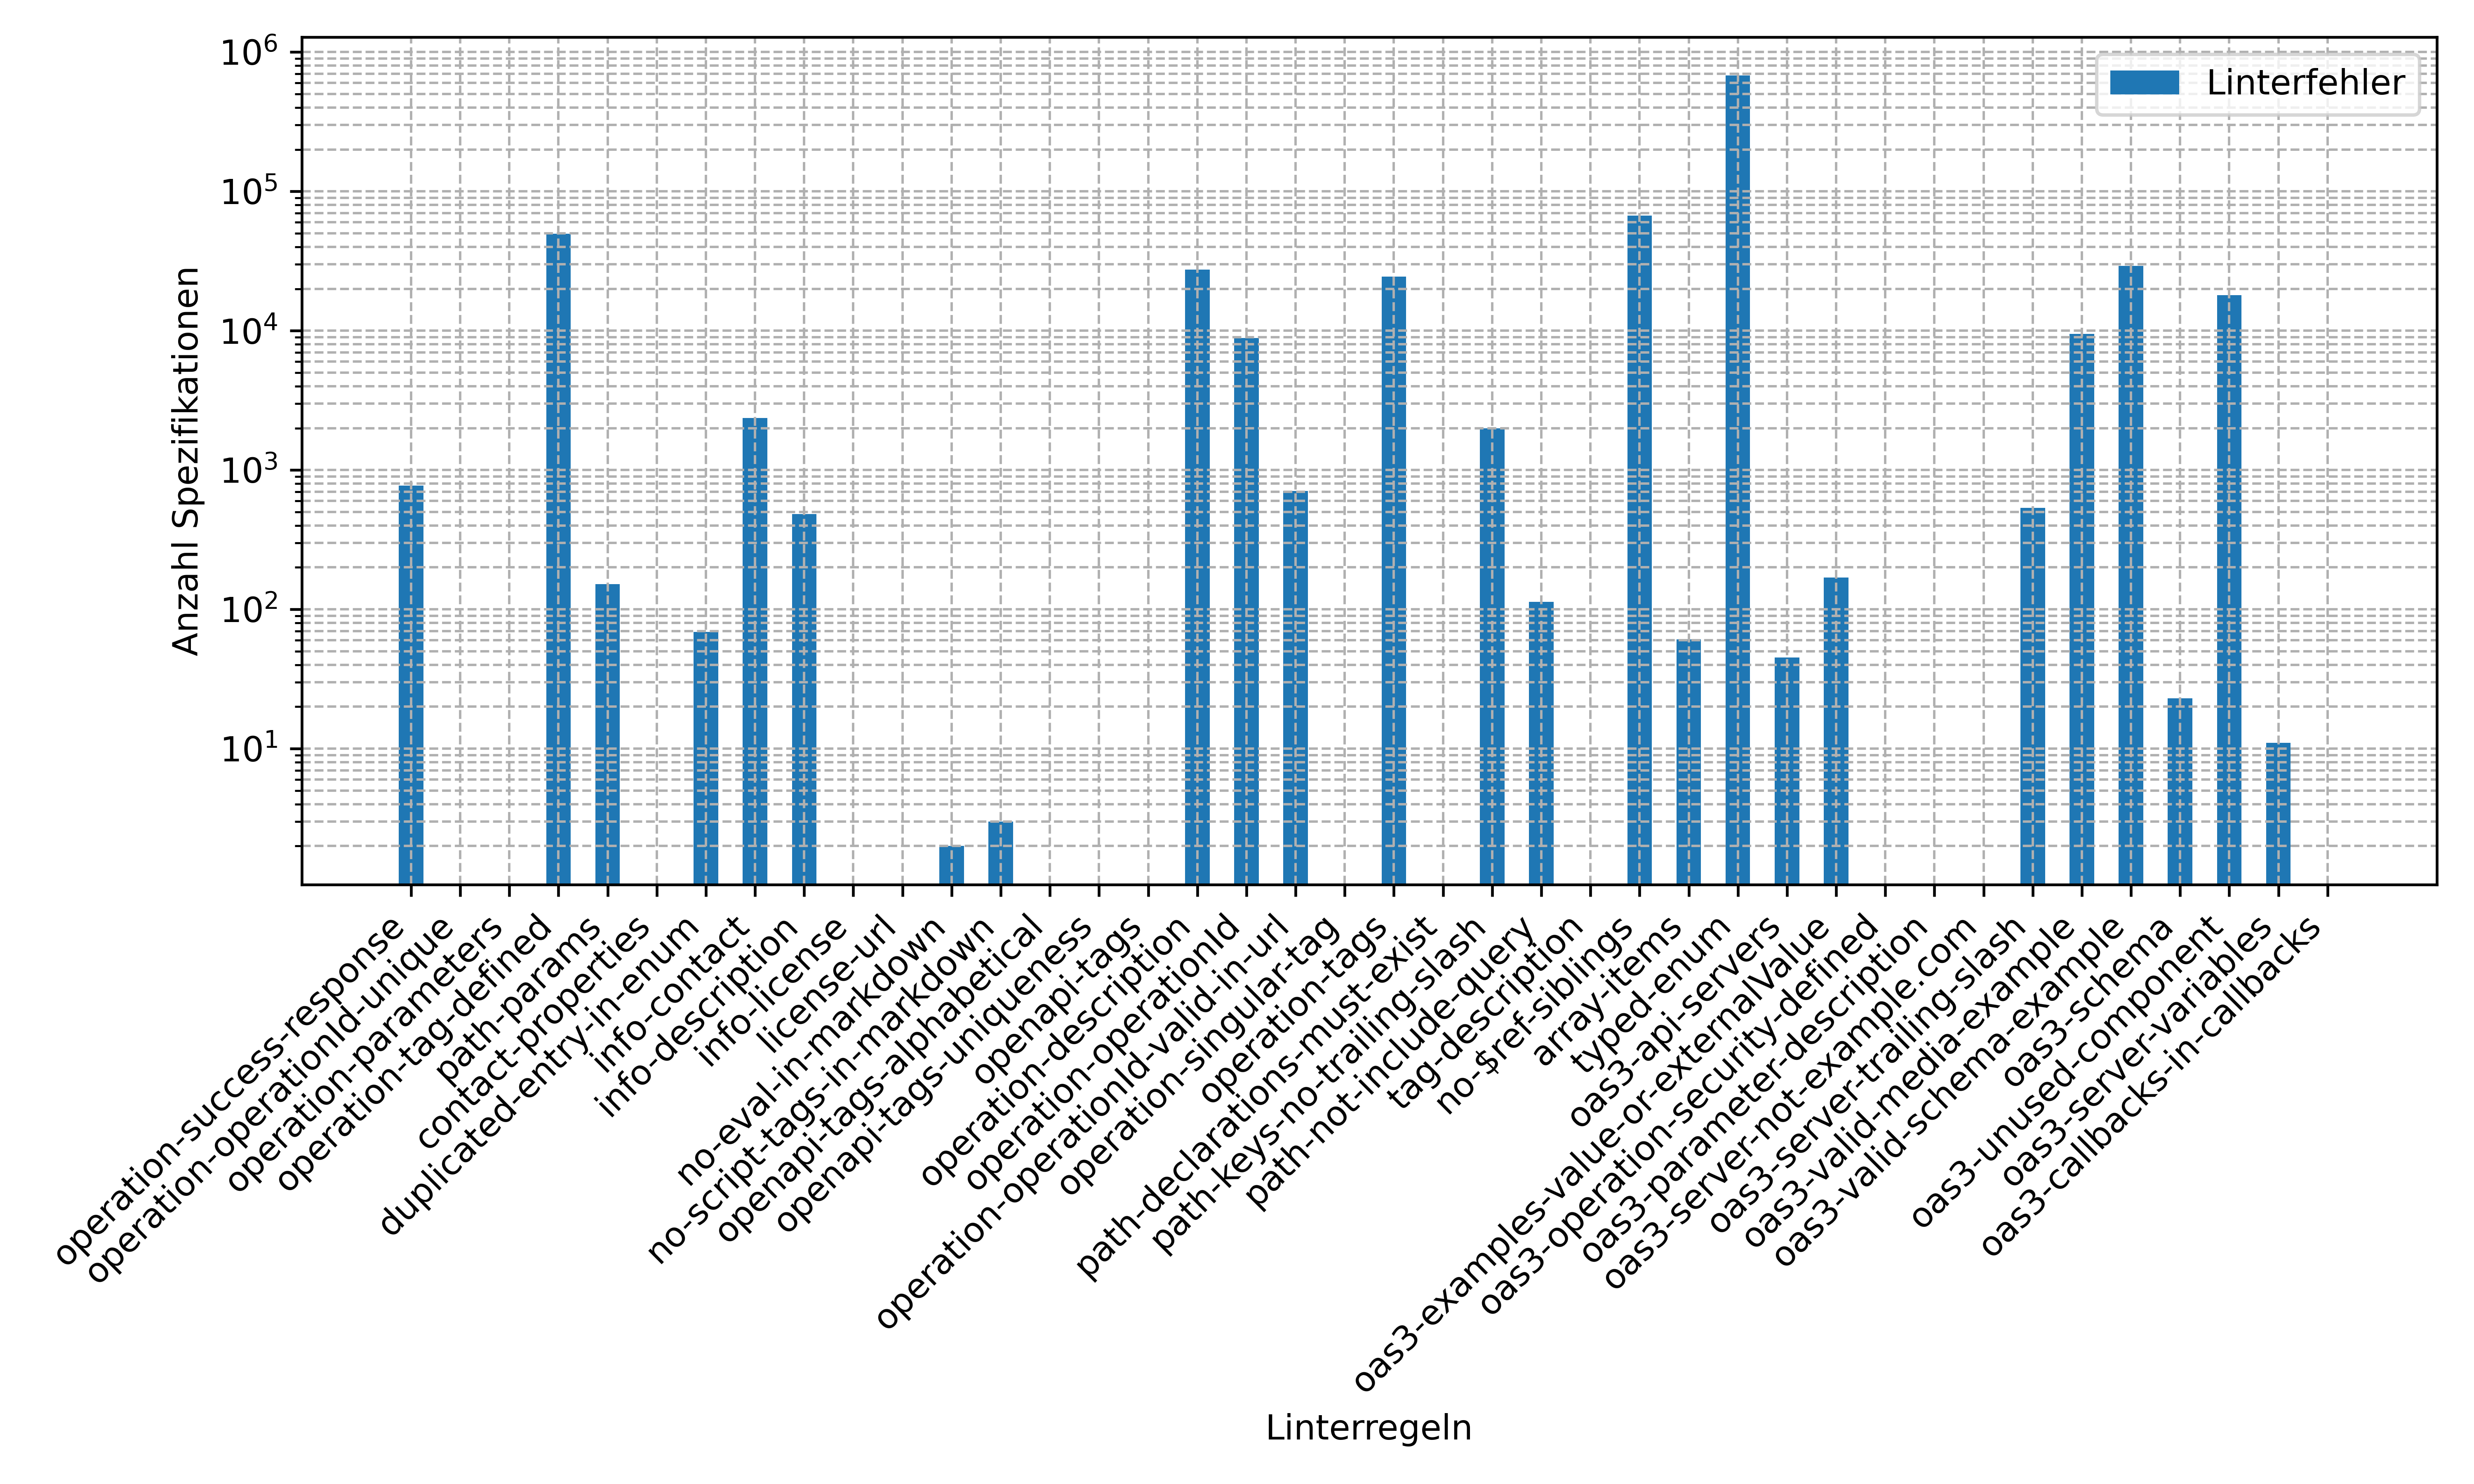
\includegraphics[width=1\linewidth]{img/totalspecthrownbarplot.png}
  \caption{Absolute Anzahl, wie viele Spezifikationen eine Linterregel ausgelöst haben}
  \label{fig:totalspecthrownbarplot}
\end{figure}


\subsubsection{Verzerrung der Linterergebnisse} \label{sec:verzerrungdesdatensatzes}
Wie in Abbildung \ref{fig:Operations} dargestellt, werden 45 \% der Spezifikationen durch den Cloudanbieter Azure.com ausgemacht. In diesem Abschnitt wird untersucht, ob es durch diese Spezifikationen eine Verzerrung im Datensatz gibt. Da bekannt ist, welche Regeln aus dem Spectral \acs{OAS} Regelwerk der Cloudanbieter zum Linten der eigenen OpenAPI Spezifikationen nimmt (siehe Tabelle \ref{tab:DeactivatedRules}), kann vermutet werden, dass die Proportion der auf von Azure.com verwendeten Linterregeln geworfenen Linterfehler niedriger ist als die aller anderen Spezifikationen.

\begin{figure}[htbp]
  \centering
  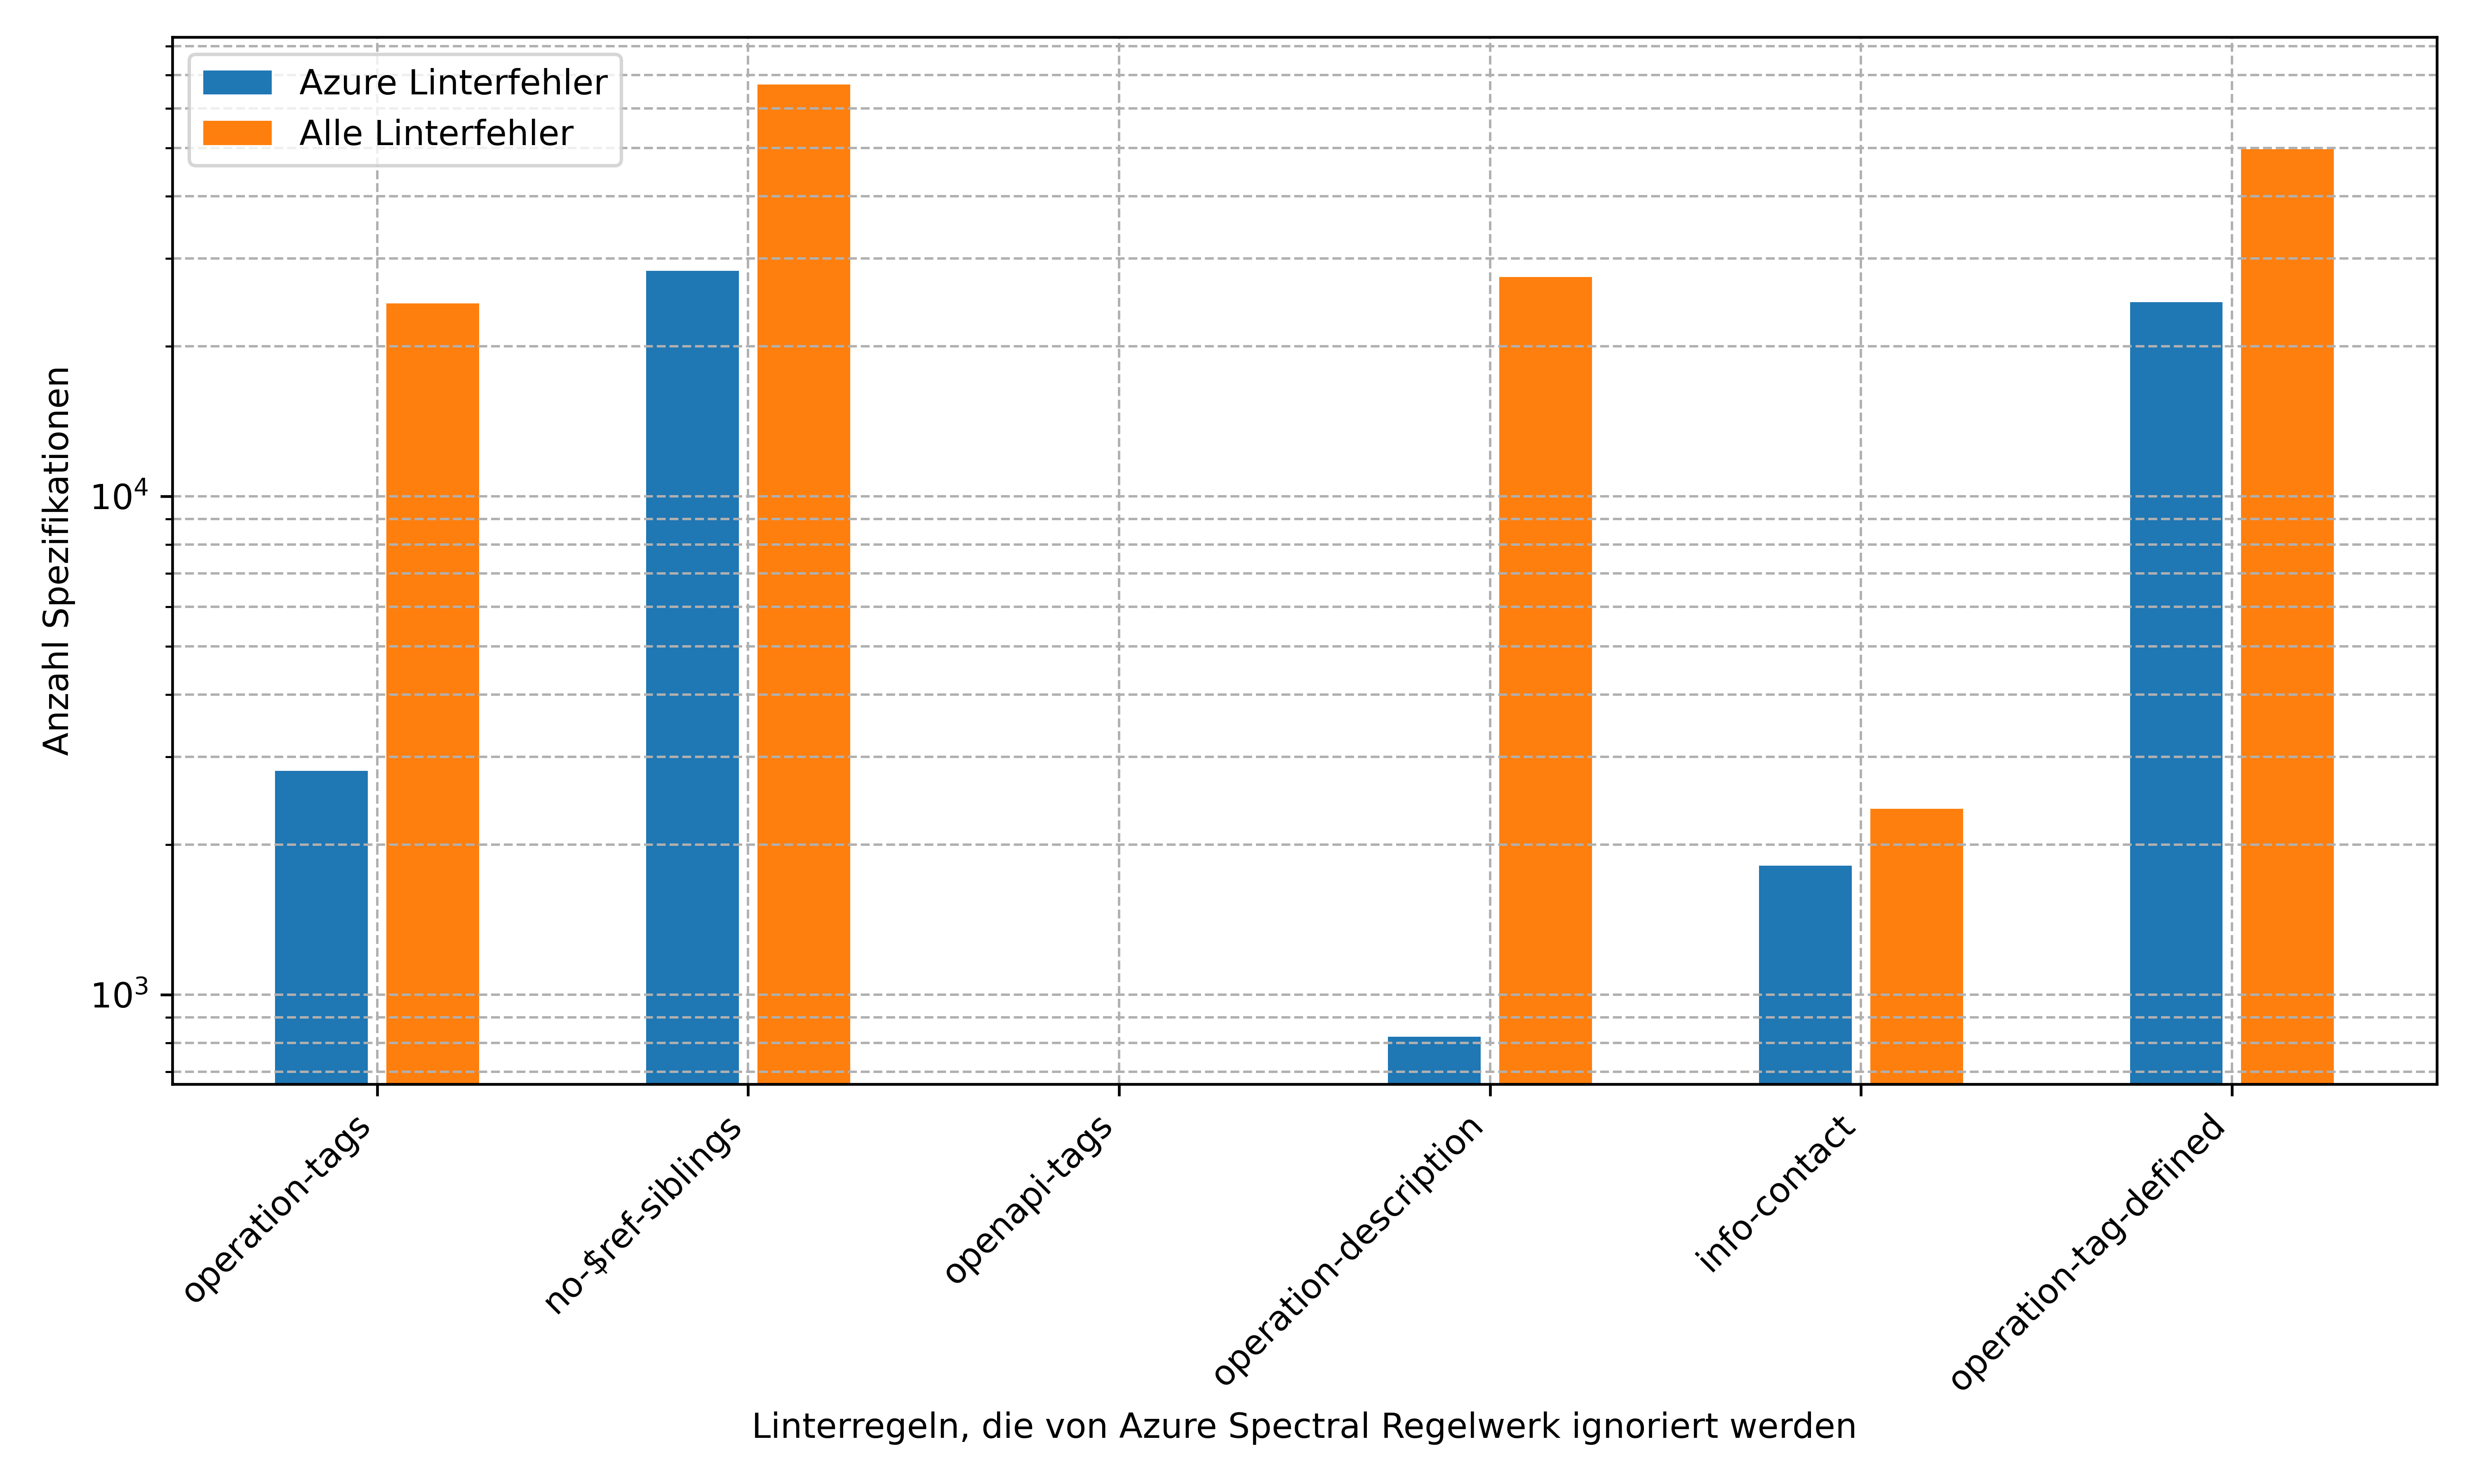
\includegraphics[width=1\linewidth]{img/azurespecthrownbarplot.png}
  \caption{Anteil der von Azure.com ausgelösten Fehler an allen Linterfehlern bei von Azure.com deaktivierten Regeln.}
  \label{fig:azurespecthrownbarplot}
\end{figure}

In Abbildung \ref{fig:azurespecthrownbarplot} wird der Anteil der Linterfehler, die von Azure.com Spezifikationen ausgelöst wurde an allen Linterfehlern gezeigt. Es lässt sich erkennen, dass die Azure.com Linterfehler bei den ausgelösten Regeln, einen großen Anteil der geworfenen Linterfehler ausmachen. Bei operation-tags, no-\$ref-siblings, info-contact und operation-tag-defined macht dieser Anzahl ca. die Hälfte aller geworfenen Linterfehler dieser Regeln aus. Dies ist erwartet, da Azure diese Regeln nicht anwendet. Für die Regeln die im Azure Spectral Regelwerk nicht deaktiviert sind, wird erwartet, dass dieser Anteil geringer ist. 

Es soll die statistische Signifikanz der Azure.com Spezifikationen auf alle Linterfehler gezeigt werden. Wir nehmen an, dass der Anteil der Azure.com Linterfehler an allen Linterfehlern normal verteilt ist. Der erwartete Wert sollte dem Anteil der Azure.com Spezifikationen an allen Spezifikationen also 0.45 entsprechen. Es wird ein studentischer t-Test gemacht für unabhängige Stichproben gemacht \parencite{mittag_statistik_2023}. Es wird gezeigt, dass der Azure.com Anteil der geworfenen Linterfehler abhängig davon ist, ob Azure.com diese Regel im Azure.com Spectral Ruleset deaktiviert.

\begin{itemize}
  \item \textbf{Gruppe 1:} Anteil an Azure.com Linterfehlern, wenn Azure die Linterregel anwendet
  \item \textbf{Gruppe 2:} Anteil an Azure.com Linterfehlern, wenn Azure die Linterregel deaktiviert
\end{itemize}

Unsere Hypothesen für die Gruppen sind:

\begin{itemize}
  \item \textbf{Nullhypothese} ($H_0$): Der durchschnittliche Anteil an Azure.com Linterfehlern unterscheidet sich nicht in beiden Gruppen  $\mu_1 = \mu_2$
  \item \textbf{Alternativhypothese} ($H_1$): Der durchschnittliche Anteil an Azure.com Linterfehlern ist niedriger, wenn Azure.com die Regel anwendet $\mu_1 < \mu_2$
\end{itemize}

Wobei $\mu_1$ und $\mu_2$ die Mittelwerte der Gesamtpopulationen repräsentieren.

Die t-Statistik wird durch folgende Formel berechnet:

\[
t=\frac{\overline{x}_1-\overline{x}_2}{\sqrt{\frac{s_1^2}{n_1}+\frac{s_2^2}{n_2}}}
\]

Wobei $\overline{x}_1$ und $\overline{x}_2$ dir Mittelwerte der Gruppen 1 und 2 darstellen, $s_1^2$ und $s_2^2$ die Varianzen der anteiligen Linterfehler und $n_1$ und $n_2$ die Größen der Gruppen sind.
Mit einem p-Wert von 0.0416, kleiner dem Signifikanzniveau $\alpha = 0.05$ ist, kann die Nullhypothese $H_0$ abgelehnt werden. Die alternative Hypothese $H_1$ wird angenommen. Dies bedeutet, dass die Anwendung der Spectral Regeln von Azure.com sich wie erwartet signifikant auf die Anteile der geworfenen Linterregeln auswirkt. Dies zeigt eine Verzerrung der Linterergebnisse durch die Anwendung des Spectral \acs{API} Linters von Azure.com. Diese Eigenschaft der Linterergebnisse wird in der Priorisierung der Ergebnisse wieder aufgegriffen. 

In \parencite{bogner_restruler_2024} ist die Größe des OpenAPI Repositories mit 2331 Spezifikationen deutlich geringer als in dieser Analyse. Anhand der Einblicke, die in dem Paper über den Datensatz gemacht werden, kann gefolgert werden, dass zu dem Zeitpunkt die Azure.com Spezifikationen noch nicht Teil des OpenAPI Directory waren. Trotz des großen Anteils der Azure.com Spezifikationen und der Verzerrung der Linterergebnisse werden hier alle Spezifikationen aus dem OpenAPI Directory als Eingabe für die Ermittlung der Linterergebnisse verwendet. Eine alternative Berechnung der Priorisierung und des Clusterings der Daten, in der Azure.com Spezifikationen nicht berücksichtigt werden findet sich im Anhang in Tabelle \ref{tab:combinedweighedpriononazure}.


\subsubsection{Auswertung der Invertierung} \label{sec:auswertungderinvertierung}
Die Invertierung zeigt das Verhältnis der geworfenen Linterregeln zu den Stellen, an denen eine Regel geworfen werden könnte. Um mit der Varianz, der Linterfehler pro Regel umzugehen, hilft diese Strategie bei der Normalisierung der Linterfehler. 

Mithilfe einer manuellen Analyse des Spectral \acs{OAS} Regelwerks wurden als Erstes die Zugehörigkeiten der Regeln zu den Klassen Inkompatibel, Single Trigger, Multi Trigger und Multi Message ermittelt. Die Zugehörigkeiten zu den Klassen Single Trigger, Multi Trigger und Multi Message werden in Tabelle \ref{tab:ruleclasses} aufgelistet.
{\footnotesize
\begin{longtable}{lll}
  \caption{\normalsize Klassifikation der Regeln}
  \label{tab:ruleclasses}
  \endfirsthead
  \endhead
  \textbf{Single Trigger} & \textbf{Multi Trigger} & \textbf{Multi Message}\\
  \hline\hline
  contact-properties & operation-success-response & operation-parameters\\
  info-contact & operation-operationId-unique & operation-tag-defined\\
  info-description & duplicated-entry-in-enum & path-params\\
  info-licence & no-eval-in-markdown & operation-description\\
  licence-url & no-script-tags-in-markdown & operation-operationId\\
  openapi-tags-alphabetical & openapi-tags-uniqueness & path-keys-no-trailing-slash\\
  oas3-api-servers & openapi-tags & path-not-include-query\\
  oas3-server-not-example.com & operation-operationId-valid-in-url & no-\$ref-siblings\\
  & operation-singular-tag & typed-enum\\
  & operation-tags & oas3-examples-value-or-external\\
  & path-declarations-must-exist & oas3-operation-security-defined\\
  & tag-description & oas3-valid-media-example\\
  & array-items & oas3-valid-schema-example\\
  & oas3-parameter-description & oas3-schema\\
  & oas3-server-trailing-slash & oas3-unused-component\\
  && oas3-server-variables\\
  && oas3-callbacks-in-callbacks\\
  \hline\hline
\end{longtable}
}

Diese wurden in einer Datei gesammelt, die als Konfiguration für das Softwaretool und für die Datenanalyse Pipeline agiert. Die Konfiguration einer Regel für das Softwaretool enthält nicht alle Attribute einer Linterregel, wie im \acs{OAS} Regelwerk. Das \acs{OAS} Regelwerk liegt zur Laufzeit des Softwaretools als eingebundenes Node Modul vor. Hieraus lassen sich nicht alle notwendigen Informationen für die Invertierung automatisiert extrahieren. Die Konfiguration, die für die Invertierung einer Regel ermittelt wurde, ist in Quellcode \ref{lst:inversionconfigexample} beispielhaft dargestellt.

\lstset{language=JavaScript}
\begin{lstlisting}[
  gobble=0,
  frame=none,
  captionpos=b,
  basicstyle=\footnotesize\ttfamily,,
  caption={Beispiel einer Regelkonfiguration für die Invertierung},
  label={lst:inversionconfigexample},
]
{
  'operation-operationId-unique': {
    formats: [],
    description: 'Every operation must have unique "operationId".',
    recommended: true,
    severity: 0,
    given: ['$.paths'],
    status: InverseStatus.MULTI_TRIGGER
  }
}
\end{lstlisting}

Algorithmus \ref{alg:invert} zur Berechnung der Summe an Selektionen eines JSONPaths wurde für jede Regel und jede Spezifikation unabhängig der Klassifizierung der Regel ausgeführt. Die Berechnung des Inversen erfolgt als Feld Mapping innerhalb der Analysepipeline. Das erzeugte Datenobjekt in den Linterergebnissen ist wie in Quellcode \ref{lst:linterresultexample} strukturiert. Abgesehen von den gezeigten Daten im Objekt werden auch die Nachrichten der Linterfehler gespeichert.

\newpage
\begin{lstlisting}[
  gobble=0,
  frame=none,
  captionpos=b,
  basicstyle=\footnotesize\ttfamily,,
  caption={Beispiel eines Ergebnisobjektes für Eine Spezifikation und Regel},
  label={lst:linterresultexample},
]
{
  'thrownMessages':40,
  'possibleMessages':48,
  'inverseStatus':'MULTI_TRIGGER'
}
\end{lstlisting}

In Tabelle \ref{tab:singletriggerinverts} wird der Mittelwert der Auslösungen für die Single Trigger Regeln gezeigt. Da die maximale Anzahl der Auslösungen für Single Trigger Regeln 1 ist, liegt der Mittelwert zwischen 0 und 1.  Die Regeln info-contact und info-description werden häufig ausgelöst (in 57 \% bzw. 12 \% der Spezifikationen). Die Regel oas3-api-servers wird selten ausgelöst (1 \% der Spezifikationen). Alle anderen Regeln werden nie ausgelöst. 

\begin{longtable}{lr}
  \caption{Mittelwert der Auslösungen von Single Trigger Regeln}
  \label{tab:singletriggerinverts}
  \endfirsthead
  \endhead
  \textbf{Regel Name} & \textbf{Mittelwert} \\ \hline\hline
  contact-properties & 0.000000 \\ 
  info-contact & 0.570358 \\ 
  info-description & 0.117021 \\ 
  info-licence & 0.000000 \\ 
  licence-url & 0.000000 \\ 
  openapi-tags-alphabetical & 0.000000 \\ 
  oas3-api-servers & 0.010880 \\ 
  oas3-server-not-example.com & 0.000000 \\ \hline\hline
\end{longtable}

Für Multi Trigger Regeln ist in Abbildung \ref{fig:multitriggerbarplot} der Mittelwert des Unterschieds zwischen geworfenen und möglichen Linterfehlern zu erkennen. Zusätzlich lässt sich an den Whiskers die Standardabweichung ablesen. An der Standardabweichung sehen wir, dass die Daten stark variieren. Bei jeder Regel ist die Standardabweichung größer als der Mittelwert (Dies lässt sich an den nach unten unbeschränkten Whiskers erkennen). Dieses Verhalten lässt sich damit begründen, dass keine der Regeln in der Mehrheit der Spezifikationen ausgelöst wird. Der Median aller Multi Trigger Regeln ist 0 (siehe \ref{tab:totalthrownerrors}). Wie auch bei den Single Trigger Regeln können wir ablesen, dass einige Regeln keinen einzigen Fehler ausgelöst haben. Das sind bei den Multi Trigger Regeln operation-operationId-unique, openapi-tags-uniqueness, openapi-tags, operation-singular-tags, path-declaration-must-exist, tag-description und oas3-parameter-description. Ein semantischer Zusammenhang dieser Regeln lässt sich nicht erkennen. In 14 / 15 Fällen ist der Mittelwert der geworfenen Linterregeln pro Spezifikation unter 1. Ausschließlich die Regel operation-tags wird im Schnitt mehr als ein Mal pro Spezifikation geworfen. 

\begin{figure}[htbp]
  \centering
  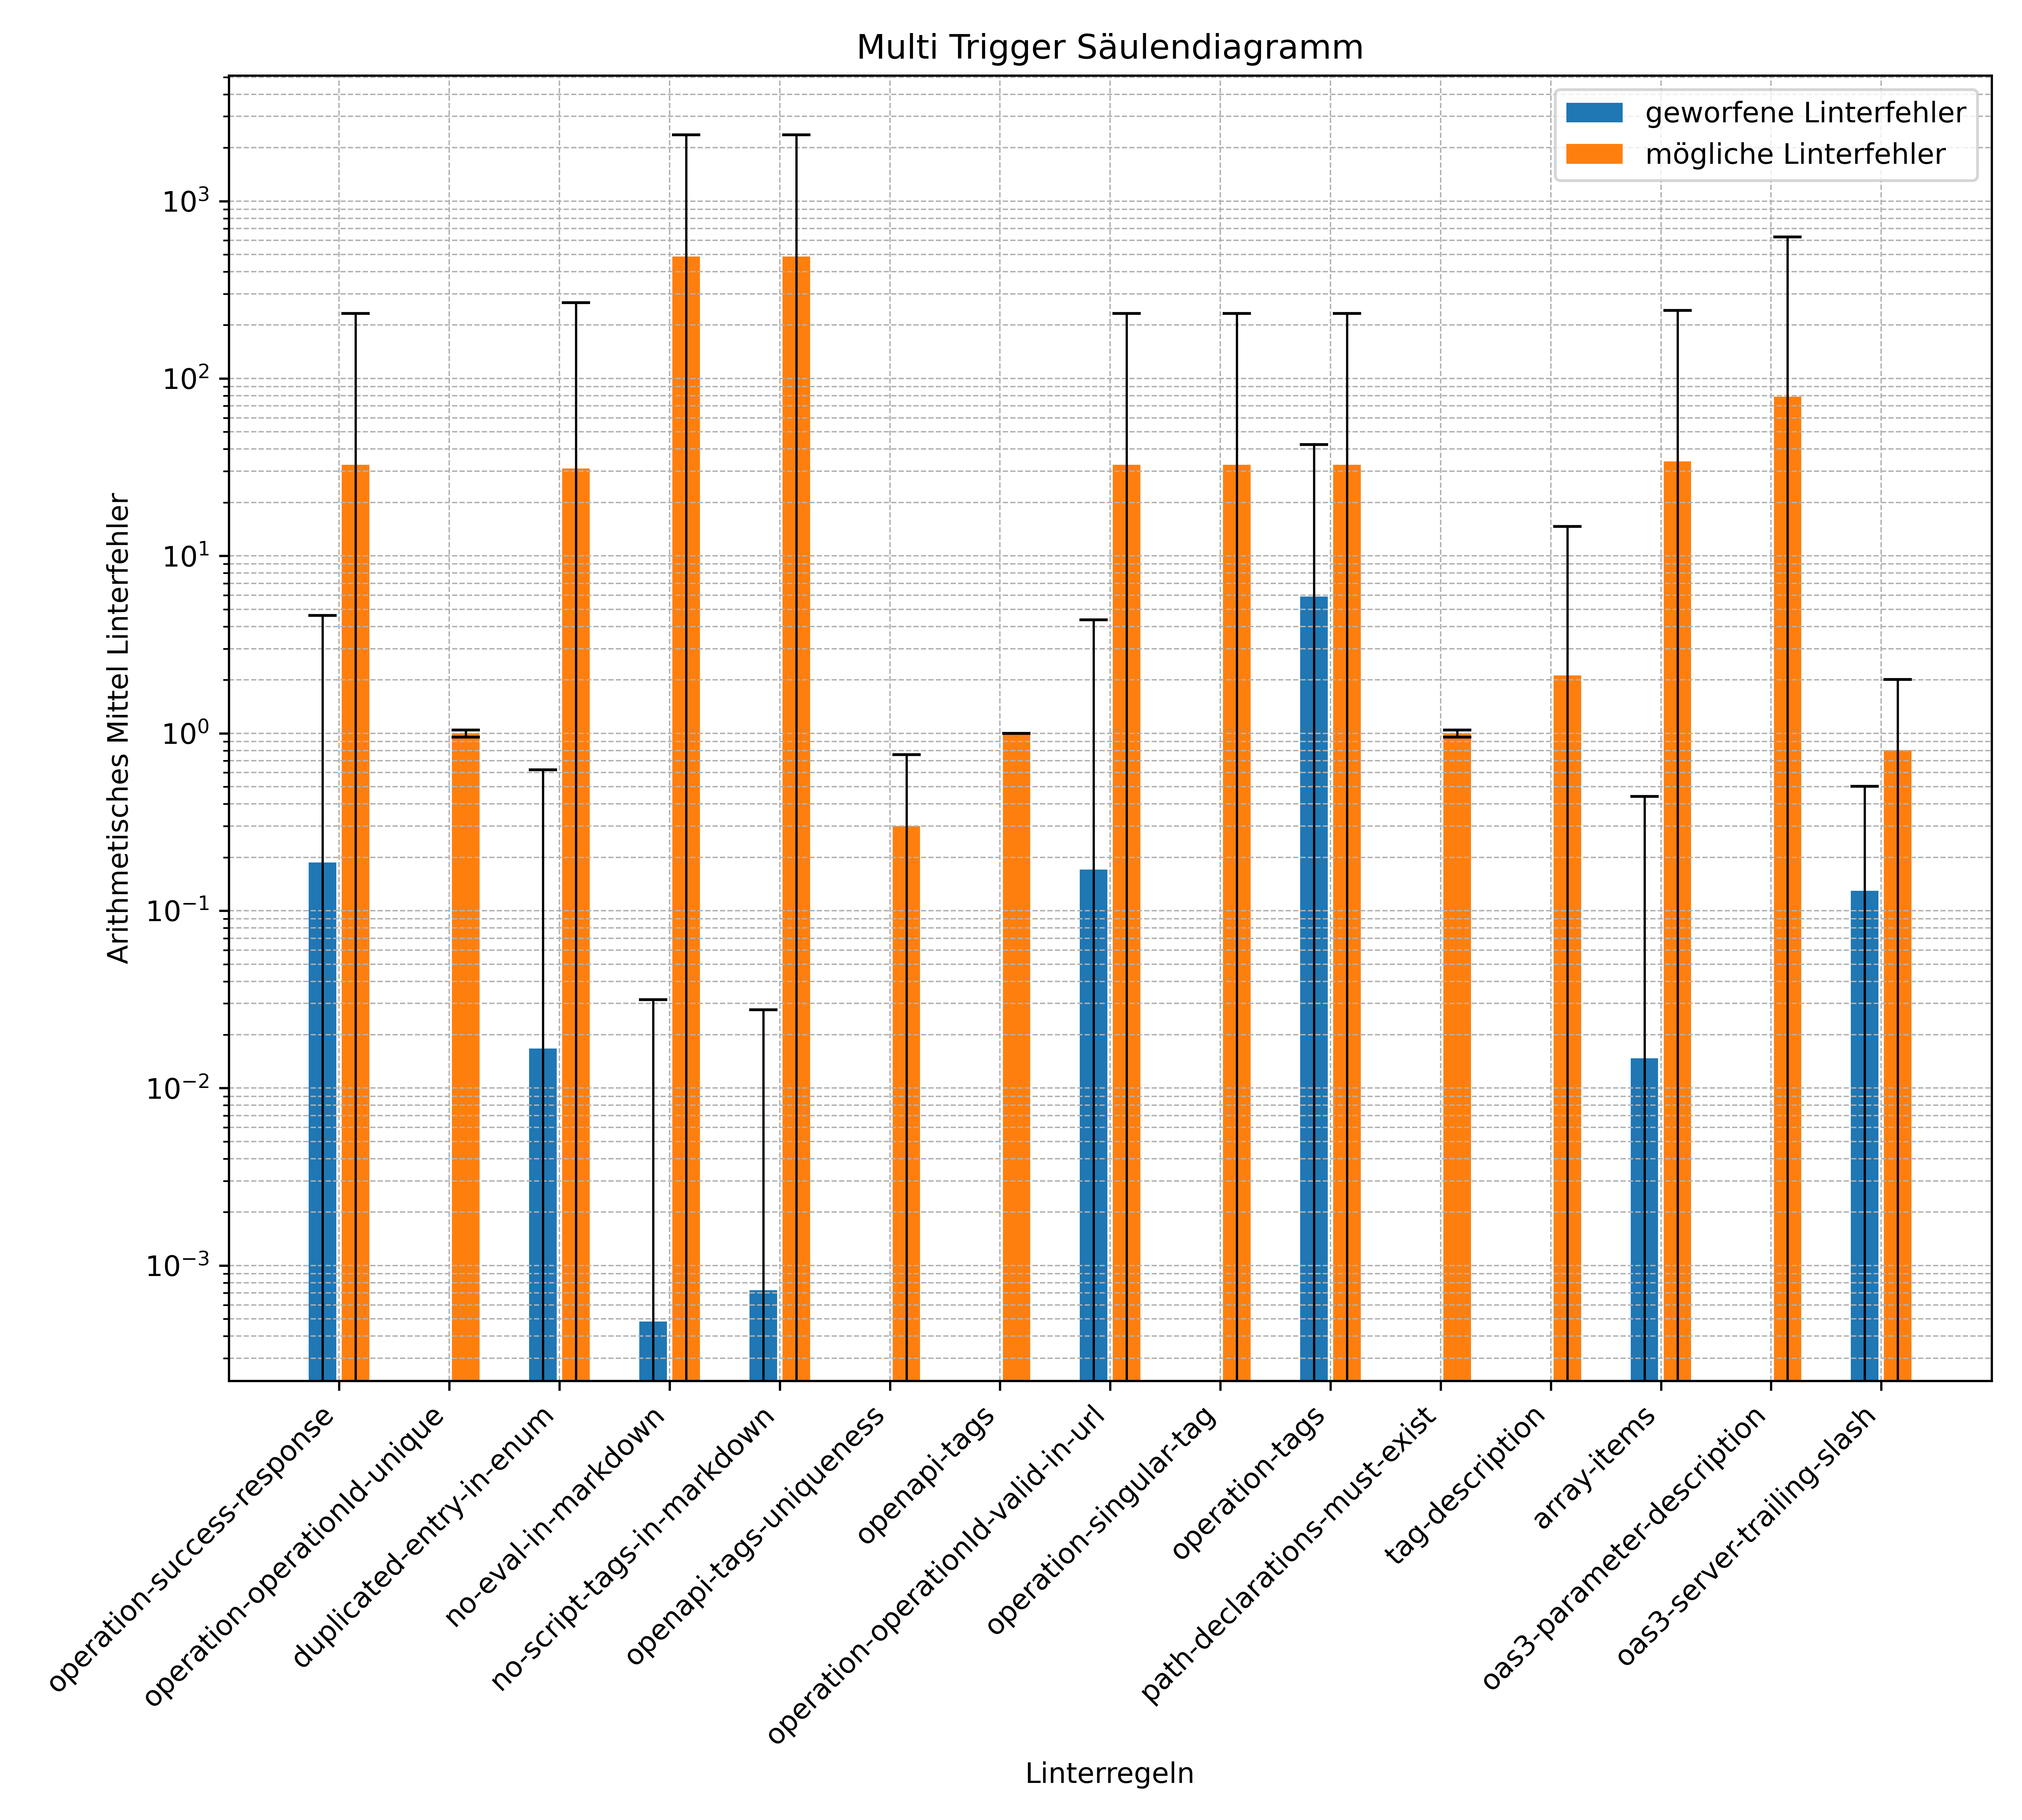
\includegraphics[width=1\linewidth]{img/multitriggerbarplot.png}
  \caption{Mittelwerte der tatsächlich geworfenen Linterfehler und möglicher Linterfehler pro Multi-Trigger Regel.}
  \label{fig:multitriggerbarplot}
\end{figure}

Die Verteilung der invertierten Häufigkeit der geworfenen Linterfehler ist für alle Regeln, die mindestens einmal ausgelöst werden, in Abbildung \ref{fig:boxplotcleanmultitrigger} gezeigt. Da der Median für diese Linterregeln gleich 0 ist und so Verteilungen nur schwer sichtbar sind, werden in dieser Visualisierung Spezifikationen, die nicht gegen eine Regel verstoßen, herausgefiltert.

Gegen die Regeln no-eval-in-markdown und no-script-tags-in-markdown, die semantisch sehr ähnlich sind, wird bei Linterfehlern nur in geringen Anteilen gegen die Regel verstoßen. Die Perzentile, Whiskers und der Median sind nahe bei null. Die Regeln operation-success-response, duplicated-entry-in-enum und array-items zeigen eine weitere Verteilung und damit eine höhere Abweichung der relativen Verstöße. Dies deutet darauf hin, dass diese Regeln auch innerhalb von einzelnen Spezifikationen nicht konsistent eingehalten werden. Die Regeln operation-operationId-valid, operation-tags und oas3-server-trailing-slash tendieren alle zu einem hohen Medianwert. Dies zeigt, dass wenn gegen die Regel verstoßen wird, dieser Verstoß konsistent in der gesamten Spezifikation zu sehen ist. Bei der Regel operation-tags ist das so eindeutig, dass Quartile der Verteilung visuell nicht zu erkennen sind. Lediglich Ausreißer sind sichtbar.

Für Multi-Message Regeln war es nicht möglich mit dem gewählten generalisierenden Ansatz Invertierungen zu berechnen. Die Anzahl der pro JSONPath Selektion möglicher Linterfehler ist teilweise abhängig von der Größe der OpenAPI Spezifikation oder von weiteren eingebundenen Softwarebibliotheken\footnote{Dies ist bei der Regel oas3-schema der Fall, in der eine Drittanbieter Bibliothek eingebunden wirft, die die Validität des Schemas mit der OpenAPI Spezifikation validiert. Die Anzahl der möglichen Fehler zu ermitteln ist nicht möglich.}. Dies macht eine aufwendige Regel spezifische Invertierung erforderlich, die im Rahmen dieser Arbeit nicht möglich ist.

\begin{figure}[htbp]
  \centering
  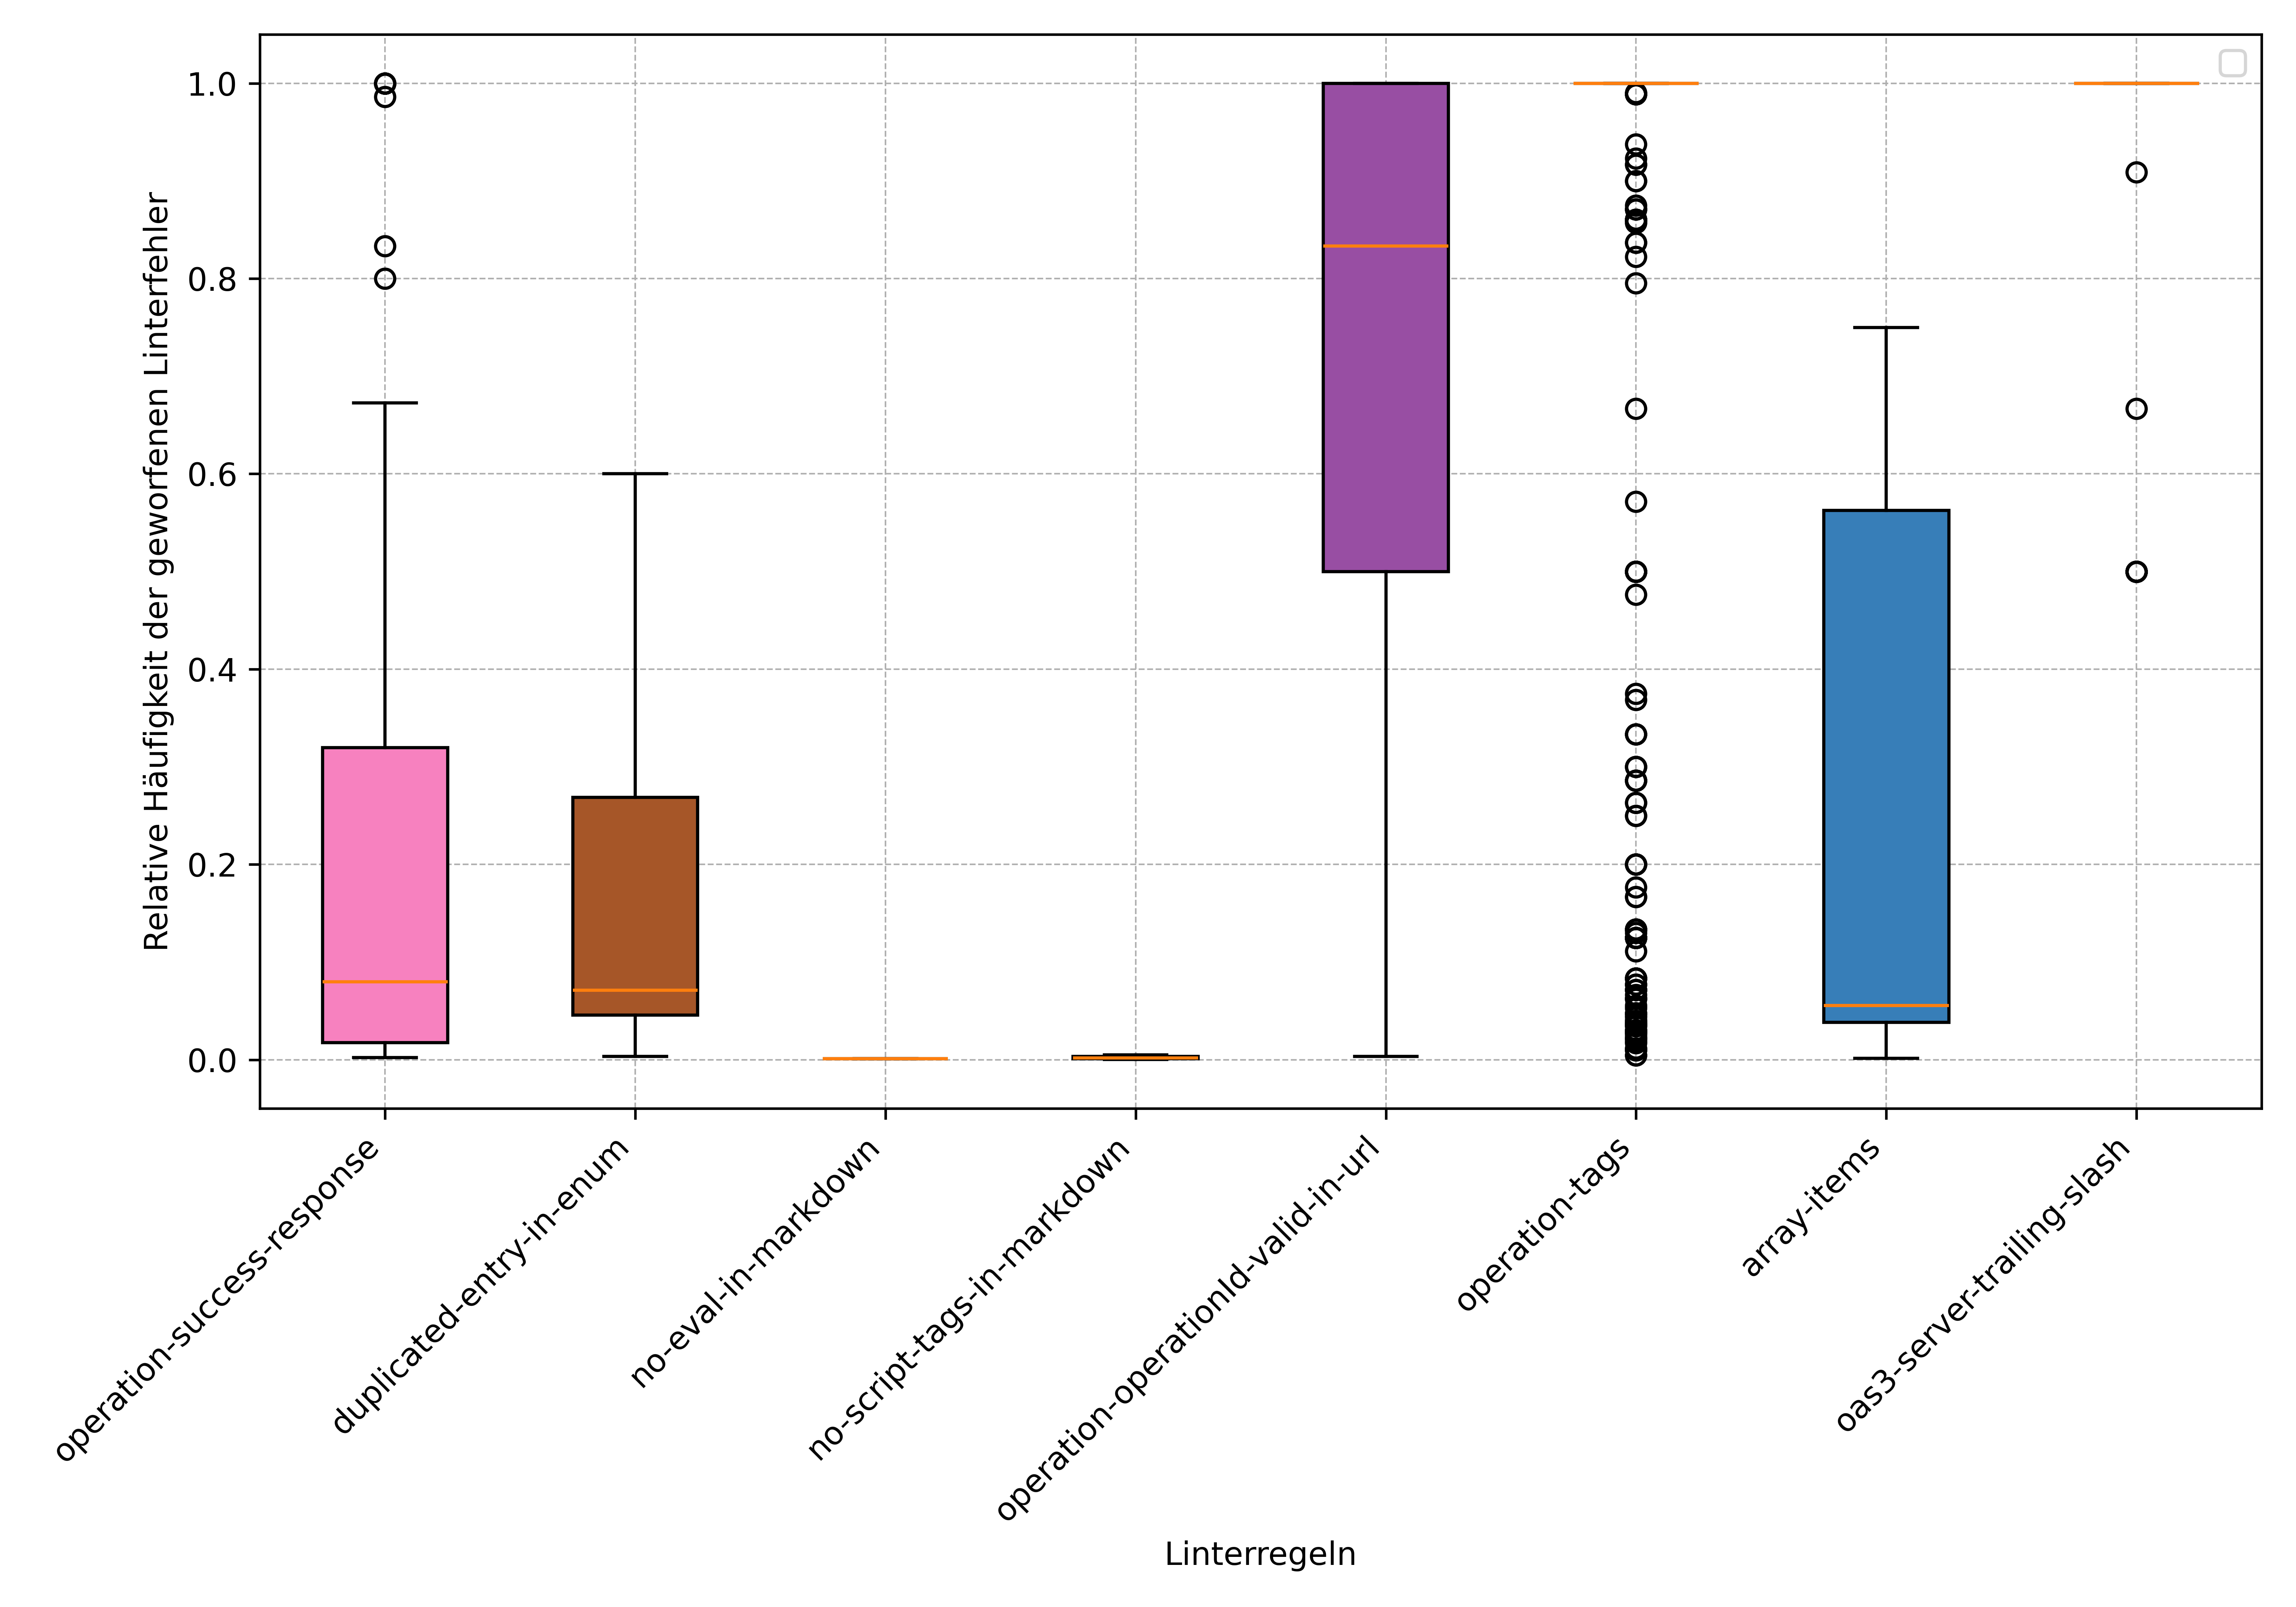
\includegraphics[width=1\linewidth]{img/boxplotcleanmultitrigger.png}
  \caption{Boxplot von Multi Trigger Regeln, wenn min. 1 Fehler geworfen wurde. Nicht triggernde Spezifikationen wurden  herausgefiltert.}
  \label{fig:boxplotcleanmultitrigger}
\end{figure}

Aus den Invertierungen lassen sich viele Informationen ablesen, die direkte Implikationen zu der Relevanz einer Regel für die Spezifikationen zulassen. Dies kann zum Beispiel in Abbildung \ref{fig:boxplotcleanmultitrigger} anhand der Konsistenz innerhalb der Spezifikationen beobachtet werden. Die Invertierung lässt sich mit der Implementierung dieser Arbeit jedoch nur für Single Trigger und Multi Trigger Regeln durchführen. Für Multi Message Regeln lassen sich diese Werte nicht ermitteln. Um trotzdem Aussagen zur Priorisierung des Spectral \acs{OAS} Regelwerks zu machen, wird in folgendem Abschnitt nur die Boolean Matrix über Vorkommnisse der Regeln und Spezifikationen betrachtet, die aussagt, ob eine Spezifikation eine Regel ausgelöst hat. Die Anzahl der Auslösungen spielt dort keine Rolle. Diese Methode ist auch unspezifisch gegenüber der Größe der Spezifikationen und lässt keine Verzerrung in Richtung großer oder kleiner Spezifikationen zu. Außerdem ist die Methode indifferent gegenüber der Regelart. Single Trigger, Multi Trigger und Multi Message Regeln können auf diese Repräsentation abgebildet werden.


\subsection{Priorisierung} \label{sec:priorisierung}
In diesem Kapitel werden die Ergebnisse der Priorisierung vorgestellt. Die Ausgangsdaten für die Priorisierungen sind ausschließlich Wahrheitswerte. Erste manuelle Einschätzungen der Relevanz konnten in der Auswertung der Invertierung gesehen werden. 


\subsubsection{Relevanz Frequenz} \label{sec:iversesfrequenzscoring}
Das Scoring der Relevanz nach \acl{IDF} ist in Tabelle \ref{tab:combinedweighedprioritized} in der Spalte $R_\text{Frequenz}$ abgebildet. Der Graph der $\text{Relevanz}_\text{Frequenz}(r)$ Funktion hat eine hyperbelähnliche Form. Regeln die null oder ein Mal ausgelöst werden, werden beide auf die Priorität 1 abgebildet. Dieses Verhalten lässt sich bei der Regel no-eval-in-markdown beobachten. Insgesamt werden 16 Regeln mit 1 priorisiert. Vier Regeln werden mit 0,1 - 0.4 bewertet. Jeweils Acht Regeln fallen auf die Größenordnungen 0.01 - 0.1, 0.001 - 0.01, 0.0001 - 0.001.


\subsubsection{Relevanz Diversität} \label{sec:diversitätsscoring}
Eine Visualisierung der jeweils minimalen Jaccard Ähnlichkeiten und ein Hierarchisches Clustering der Regeln ist in Abbildung \ref{fig:hierarchicalclusteronbinary} dargestellt. Die Priorisierung nach $\text{Relevanz}_\text{Diversität}$ ergibt sich indirekt aus den Werten, die durch das Dendrogramm visualisiert werden. Das Dendrogramm eignet sich, um die Motivation der des $\text{Relevanz}_\text{Diversität}$ zu verdeutlichen.

In dieser Abbildung lassen sich die Regeln, die nie ausgelöst wurden, als Cluster erkennen. Ein zweites Cluster wird durch die Regeln no-eval-in-markdown, no-script-tags-in-markdown und openapi-tags-uniqueness gebildet. Dies zeigt, dass diese Regeln von den gleichen Spezifikationen missachtet wurden. Durch die Ähnlichkeit des Auslösemusters der Regeln, die in Markdown eingebetteten Code erkennen, liegt nahe, dass diese von den gleichen Spezifikationen ausgelöst wurden. Die Einbettung von Code in die Markdownfelder ist hier eventuell intendiertes Verhalten. Die verbleibenden 22 Regeln werden im Dendrogramm in ein großes Cluster eingeteilt. Wir können erkennen, dass diese in der Regel bei Jaccard Ähnlichkeiten größer 0,8 zusammengeführt werden. Für die Linterergebnisse bedeutet dies, dass keine weiteren Trends zum Missachten bestimmter Regeln vorliegen. 

In Tabelle \ref{tab:combinedweighedprioritized} wird die Gewichtung der $\text{Relevanz}_\text{Diversität}(r)$ in Spalte $R_\text{Diversität}$ gezeigt. Auch in diesem Priorisierungsmaß werden die Regeln, die nie getriggert werden mit 0,375 am höchsten bewertet. Alle anderen Regeln sind mit einem Wert zwischen 0,02 und 0,07 bewertet.

\begin{figure}[htbp]
  \centering
  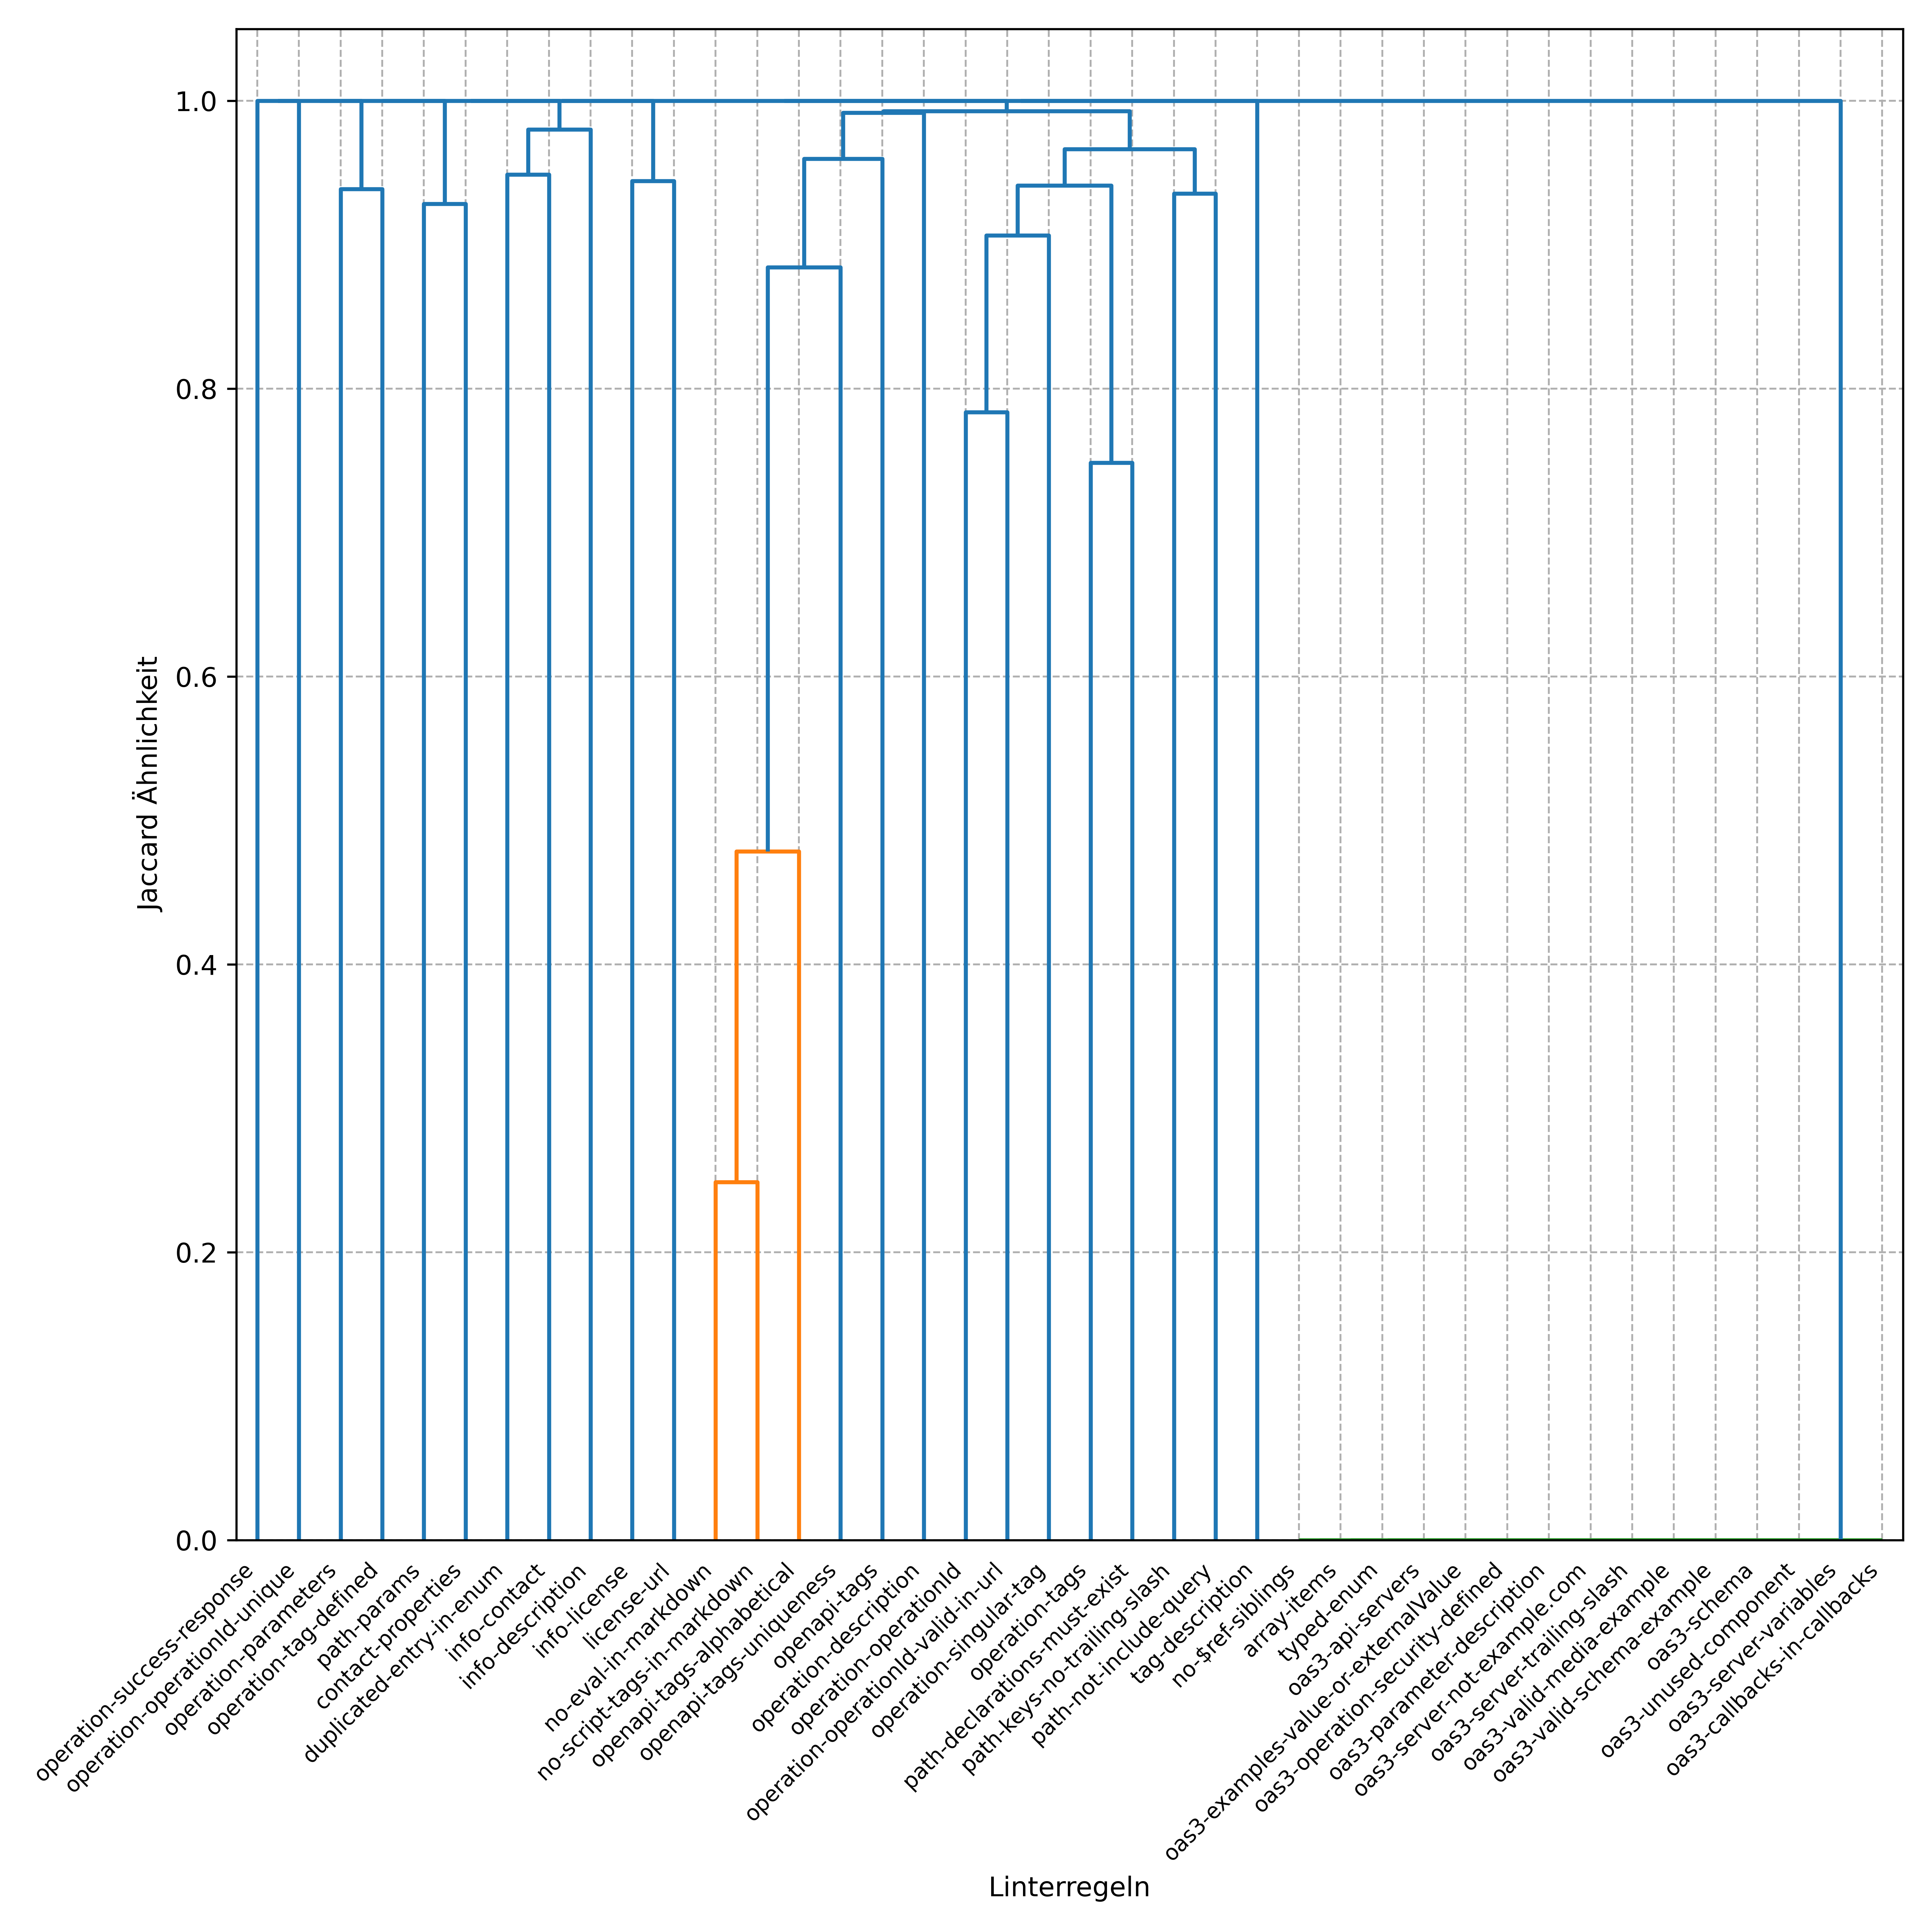
\includegraphics[width=1\linewidth]{img/hierarchicalclusteronbinary.png}
  \caption{Dendrogramm der Jaccard Ähnlichkeit der Regeln.}
  \label{fig:hierarchicalclusteronbinary}
\end{figure}


\subsubsection{Kombination der Verfahren} \label{sec:kombinationderverfahren}
Die gewichtete Kombination der Priorisierungsverfahren ist in Tabelle \ref{tab:combinedweighedprioritized} in der Spalte Kombiniert verdeutlicht. Je größer die Werte der kombinierten Priorisierung, desto relevanter ist einer Regel nach dem kombinierten Maß. Die gesamte Tabelle ist nach den Werten in dieser Spalte absteigend sortiert. Die Koeffizienten $\alpha$ und $\beta$ wurde wie folgt gewählt\footnote{Die Wahl der Koeffizienten ist nicht optimiert, sondern entspricht einer Einschätzung des Autors.}:

\[
\alpha = 0,8 ; \beta = 0,2
\]

Tabelle \ref{tab:combinedweighedprioritized} bildet das Kernstück der Datenanalyse der Arbeit. Die Tabelle aggregiert Informationen zur Priorisierung der $\text{Relevanz}_\text{Frequenz}$ und der $\text{Relevanz}_\text{Diversität}$ sowie die gewichtete Kombination der Maße und der Einteilung, basierend auf der Relevanz der Regeln in Cluster zu neuen Linterschweregraden. Dies sind alle Werte, die im Rahmen der Priorisierung der Linterregeln ermittelt werden. Die mit der Tabelle visualisierten Daten beantworten die Forschungsfragen \textbf{RQ-2} und \textbf{RQ-3}.

An den Werten der gewichteten Kombination kann erkannt werden, dass in den meisten Fällen, die $\text{Relevanz}_\text{Frequenz}$ ausschlaggebend für die Position in der Priorisierung ist. Regeln, die durch das $\text{Relevanz}_\text{Frequenz}$ sehr niedrig priorisiert wurden, werden durch die $\text{Relevanz}_\text{Diversität}$ Priorisierung teilweise aufgewertet. Die Verteilung der Relevanzen in beiden Maßen neigt stark zu den Rändern. Dies bedeutet, dass Regeln entweder hoch priorisiert werden oder sehr niedrig priorisiert werden. Um dies zu verdeutlichen ist in Abbildung \ref{fig:priodistrhist} ein Histogramm abgebildet, das die Verteilung der Priorisierungen nach den verschiedenen Maßen abbildet. Man kann erkennen, dass die niedrig priorisierten Regeln in dem Bereich von einer Relevanz von 0 bis 0,2 verteilt sind. Hoch priorisierte Regeln sind eng beieinanderliegend, da dies die Regeln umfasst, die nie ausgelöst wurden. Diese werden nach beiden Priorisierungsmaßen immer mit dem höchsten Wert bewertet. Zwischen den Randakkumulationen werden einige Regeln nach der $\text{Relevanz}_\text{Frequenz}$ im mittleren Bereich des Spektrums angesiedelt. Diese Informationen werden in der Neuverteilung der Linter Schweregrade weiterverwendet und sind für das Clustering ausschlaggebend.

\begin{figure}[htbp]
  \centering
  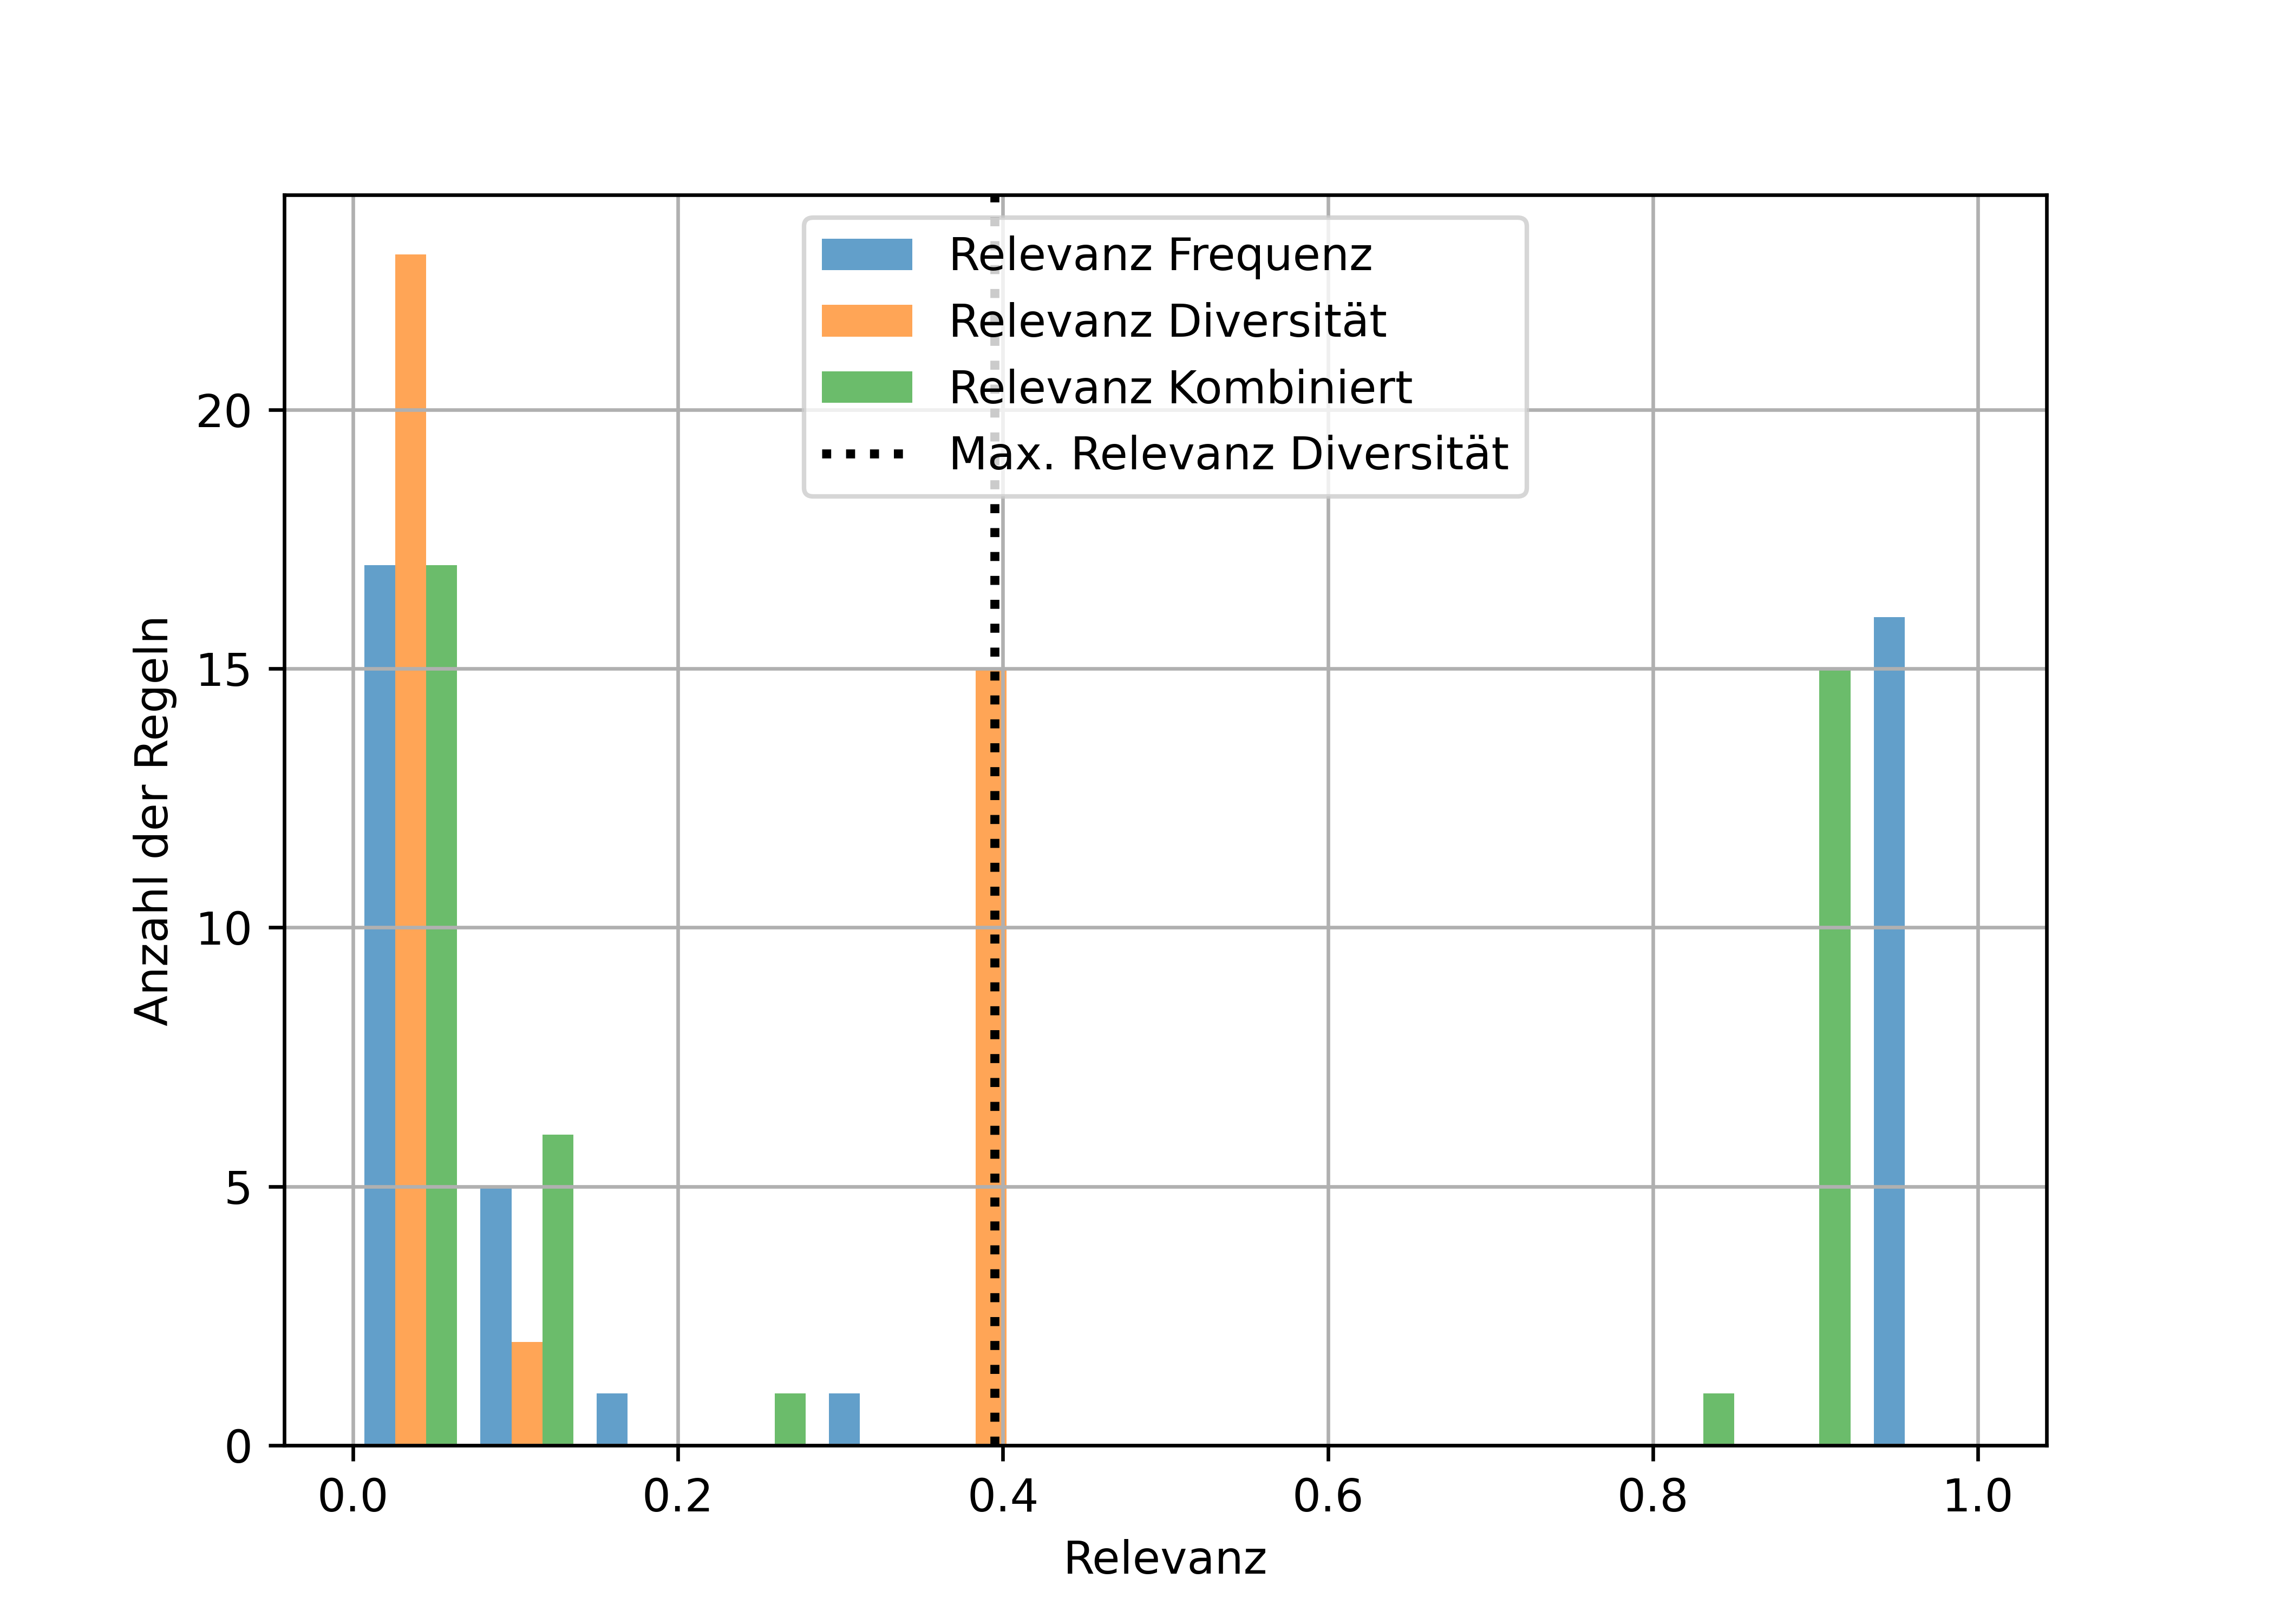
\includegraphics[width=1\linewidth]{img/priodistrhist.png}
  \caption{Histogramm Verteilung der Relevanz}
  \label{fig:priodistrhist}
\end{figure}

\newpage
{\footnotesize
\begin{longtable}{lrrrrr}
  \caption{\normalsize Relevanzmaße, gewichtete Kombination und Schweregrad Neuverteilung. Mit * markierte Regeln wurden nie ausgelöst. Horizontale Linien zeigen Grenzen zwischen Clustern}
  \label{tab:combinedweighedprioritized}
  \endfirsthead
  \endhead
  \textbf{Regel} & \textbf{$\text{R}_\text{Frequenz}$} & \textbf{$\text{R}_\text{Diversität}$} & \ \textbf{Kombiniert} & \textbf{OAS} & \textbf{Cluster} \\ \hline \hline

  operation-operationId-unique* & 1 &  0.375 & 0.875 & \texttt{hint} & \texttt{error} \\ 
  operation-parameters* & 1 &  0.375 & 0.875 & \texttt{warn} & \texttt{error} \\ 
  contact-properties* & 1 &  0.375 & 0.875 & \texttt{warn} & \texttt{error} \\ 
  openapi-tags* & 1 &  0.375 & 0.875 & \texttt{warn} & \texttt{error} \\ 
  openapi-tags-alphabetical* &  1 &  0.375 & 0.875 & \texttt{warn} & \texttt{error} \\ 
  openapi-tags-uniqueness* &  1 &  0.375 & 0.875 & \texttt{error} & \texttt{error} \\ 
  licence-url* &  1 &  0.375 & 0.875 & \texttt{warn} & \texttt{error} \\ 
  info-licence* & 1 &  0.375 & 0.875 & \texttt{warn} & \texttt{error} \\ 
  oas3-server-not-example.com* &  1 &  0.375 & 0.875 & \texttt{warn} & \texttt{error} \\ 
  oas3-operation-security-defined* &  1 &  0.375 & 0.875 & \texttt{warn} & \texttt{error} \\ 
  oas3-parameter-description* & 1 & 0.375 & 0.875 & \texttt{warn} & \texttt{error} \\ 
  oas3-callbacks-in-callbacks* &  1 &  0.375 & 0.875 & \texttt{warn} & \texttt{error} \\ 
  path-declarations-must-exist* & 1 &  0.375 & 0.875 & \texttt{warn} & \texttt{error} \\ 
  operation-singular-tag* & 1 &  0.375 & 0.875 & \texttt{warn} & \texttt{error} \\ 
  tag-description* &  1 &  0.375 & 0.875 & \texttt{warn} & \texttt{error} \\ 
  no-eval-in-markdown &  1 &  0.025194 & 0.805039 & \texttt{warn} & \texttt{error} \\ \hline
  no-script-tags-in-markdown & 0.333333 &  0.026171 & 0.271901 & \texttt{warn} &  \texttt{warn} \\ 
  duplicated-entry-in-enum & 0.166667 &  0.028361 & 0.139006 & \texttt{warn} &  \texttt{warn} \\ 
  oas3-schema &  0.142857 &  0.029349 & 0.120156 & \texttt{hint} &  \texttt{warn} \\ 
  array-items &  0.111111 &  0.029397 & 0.094768 & \texttt{hint} &  \texttt{warn} \\ 
  path-not-include-query & 0.090909 &  0.034471 & 0.079621 & \texttt{warn} &  \texttt{warn} \\ 
  oas3-server-variables &  0.090909 &  0.027007 & 0.078129 & \texttt{hint} &  \texttt{warn} \\ 
  oas3-examples-value-or-externalValue & 0.083333 &  0.032167 & 0.073100 & \texttt{warn} &  \texttt{warn} \\ \hline
  operation-operationId-valid-in-url & 0.024390 &  0.035357 & 0.026584 & \texttt{warn} &  \texttt{hint} \\ 
  typed-enum & 0.022222 &  0.036551 & 0.025088 & \texttt{warn} &  \texttt{hint} \\ 
  oas3-api-servers & 0.022222 &  0.031494 & 0.024077 & \texttt{warn} &  \texttt{hint} \\ 
  operation-success-response & 0.017241 &  0.038016 & 0.021396 & \texttt{warn} &  \texttt{hint} \\ 
  path-params &  0.012658 &  0.040815 & 0.018290 & \texttt{hint} &  \texttt{hint} \\ 
  info-contact & 0.000424 &  0.074276 & 0.015194 & \texttt{warn} &  \texttt{hint} \\ 
  operation-tag-defined &  0.000435 &  0.073718 & 0.015092 & \texttt{warn} &  \texttt{hint} \\ 
  oas3-valid-media-example & 0.006289 &  0.049300 & 0.014892 & \texttt{hint} &  \texttt{hint} \\ 
  no-\$ref-siblings & 0.000457 &  0.067871 & 0.013940 & \texttt{hint} &  \texttt{hint} \\ 
  path-keys-no-trailing-slash &  0.006536 &  0.042196 & 0.013668 & \texttt{warn} &  \texttt{hint} \\ 
  operation-description &  0.001669 &  0.059269 & 0.013189 & \texttt{warn} &  \texttt{hint} \\ 
  oas3-valid-schema-example &  0.002347 &  0.054599 & 0.012798 & \texttt{hint} &  \texttt{hint} \\ 
  oas3-unused-component &  0.000992 &  0.059835 & 0.012761 & \texttt{warn} &  \texttt{hint} \\ 
  operation-operationId &  0.002632 &  0.052863 & 0.012678 & \texttt{warn} &  \texttt{hint} \\ 
  info-description & 0.002066 &  0.049029 & 0.011459 & \texttt{warn} &  \texttt{hint} \\ 
  operation-tags & 0.001096 &  0.046861 & 0.010249 & \texttt{warn} &  \texttt{hint} \\ 
  oas3-server-trailing-slash & 0.001927 &  0.043539 & 0.010249 & \texttt{warn} &  \texttt{hint} \\ \hline\hline
\end{longtable}
}


\subsubsection{Clustering} \label{sec:analclustering}
In Tabelle \ref{tab:combinedweighedprioritized} kann man die Zugehörigkeit der Regeln zu Clustern, die Linter Schweregraden zugeordnet werden, sehen. Die Clusterzugehörigkeiten werden durch die Spalte Cluster und durch horizontale Linien in der Tabelle sichtbar. In Abbildung \ref{fig:clusterprioscatter} wird die Priorisierung der Linterregeln auf einem Scatterplot gezeigt. Für die Clusterzuordung wurde das k-means Verfahren verwendet. Ein Scatterplot eignet sich gut, um diese Clusterzugehörigkeiten im Zweidimensionalen Raum visuell darzustellen. Die Priorisierungsmaße sind die Dimensionen.

Zusätzlich werden auf dem Scatterplot Voronoi Regionen gezeigt, die visualisieren, welche Regionen einem Cluster zugeordnet werden können \parencite{klein_algorithmische_2022}. Da die Daten dicht beieinanderliegen, kann mit dieser Methode die Verteilung der Cluster über den gesamten Relevanzraum gezeigt werden. Es ist sichtbar, dass die Cluster auch ausschließlich auf dem $\text{Relevanz}_\text{Frequenz}$ Maß aufgestellt werden könnten. Die Cluster unterscheiden sich klar auf der in ihren $\text{Relevanz}_\text{Frequenz}$ Werten. Die $\text{Relevanz}_\text{Diversität}$ Werte befinden sich bis auf die Regeln, die nie ausgelöst werden sehr dicht beieinander. Die $\text{Relevanz}_\text{Diversität}$ Werte verursachen die Schräge der Grenzen der Voronoi Regionen. Diese teilen die Fläche der möglichen Priorisierungen in drei Regionen, die um die Clustermittelpunkte (Centroiden) angeordnet sind.

\begin{figure}[htbp]
  \centering
  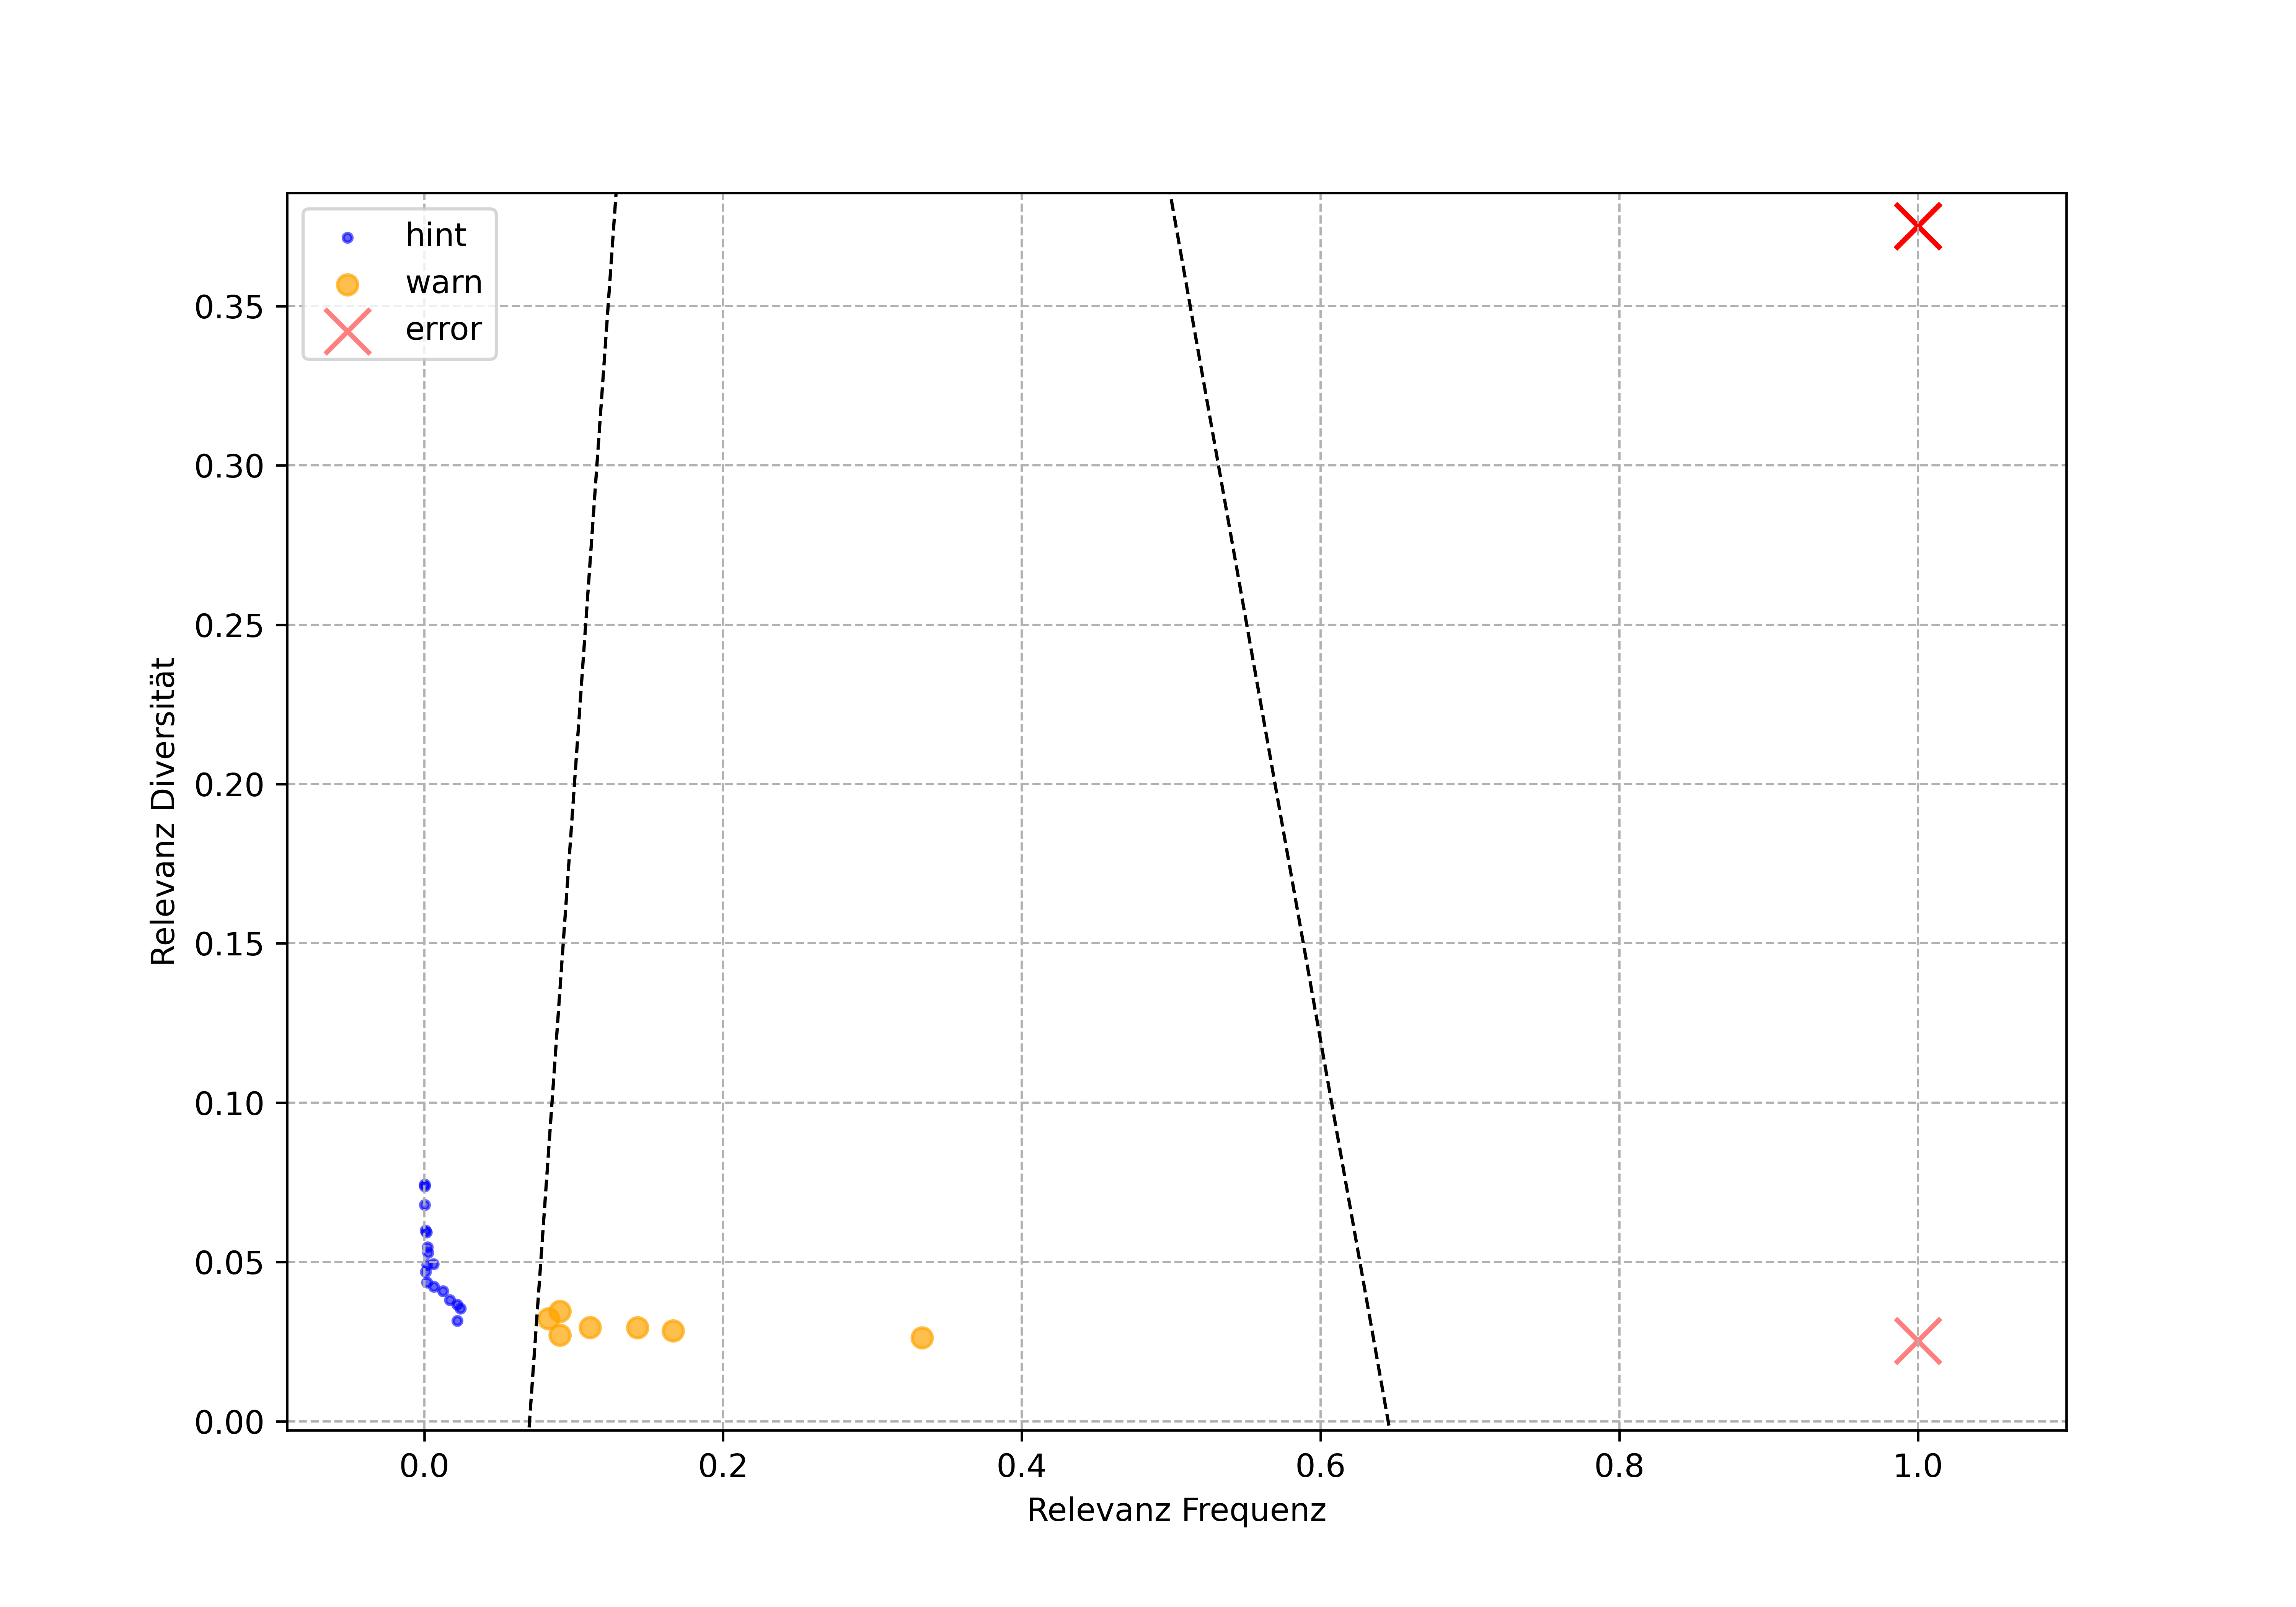
\includegraphics[width=1\linewidth]{img/clusterprioscatter.png}
  \caption{Scatterplot der Priorisierungsmaße mit Voronoi Regionen.}
  \label{fig:clusterprioscatter}
\end{figure}

Nach der Neuverteilung der Linter Schweregrade durch das k-means Clustering haben viele der Linterregeln eine Zuordnung zu einem anderen Schweregrad als im Spectral OAS Regelwerk. Die Neuverteilungen werden in Tabelle \ref{tab:severityreassignments} gezeigt. Nur in einem Fall (operation-operationId-unique) werden zwei Linter Schweregrade übersprungen. Diese Regel wurde nie ausgelöst. Die größten Verschiebungen finden zwischen \texttt{warn} und \texttt{error} bzw. \texttt{error} statt. Der Schweregrad \texttt{warn} wird durch den Spectral Linter standardisiert zugewiesen, wenn keine explizite Einteilung durch das Regelwerk vorgenommen wurde. Seit Version 5.0 ist die Standardkonfiguration des Spectral \acs{API} Linters, dass nur Regeln mit dem Schweregrad \texttt{error} einen Laufzeitfehler mit einem Statuscode von 1 auslösen\footnote{Erwähnt in der Spectral CLI Dokumentation: \href{https://meta.stoplight.io/docs/spectral/9ffa04e052cc1-spectral-cli}{https://meta.stoplight.io/docs/spectral/9ffa04e052cc1-spectral-cli}}. Mit 15 Regeln, die durch das Clustering auf den Schweregrad  \texttt{error} gestellt werden, ist die Anzahl von Regeln, die den Linter mit Standardeinstellungen zum Fehlschlagen bringen, bedeutend höher. Im \acs{OAS} Regelwerk sind die meisten Regeln, dem Schweregrad \texttt{warn} zugewiesen. Vier Regeln werden im \acs{OAS} Regelwerk mit \texttt{hint} bewertet, die in der Neuverteilung eine oder mehrere Schweregrade nach oben rutschen. Diese Regeln sollen in der Interpretation semantisch untersucht werden, ob es sich um Regeln handelt, die im \acs{OAS} Regelwerk falsch klassifiziert wurden oder, ob es sich um seltene Randfälle handelt, die im APIs.guru Datensatz nie vorgekommen sind. Im ersten Fall wäre die Einordnung als \texttt{error} korrekt. Letzteres würde die Klassifizierung als \texttt{error} eher überflüssig erscheinen lassen.

\begin{longtable}{llr}
  \caption{Neuverteilungen der Linter Schweregrade}
  \label{tab:severityreassignments}
  \endfirsthead
  \endhead
  \textbf{Schweregrad \acs{OAS}} & \textbf{Schweregrad Cluster} & \textbf{Anzahl} \\ \hline \hline
  \texttt{hint} & \texttt{hint} & 4 \\
  \texttt{warn} & \texttt{warn} & 4 \\
  \texttt{error} & \texttt{error} & 1 \\
  \texttt{warn} & \texttt{error} & 13 \\
  \texttt{warn} & \texttt{hint} & 12 \\
  \texttt{hint} & \texttt{warn} & 3 \\
  \texttt{hint} & \texttt{error} & 1 \\
  \hline\hline
\end{longtable}

Ob den Ergebnissen die durch die Priorisierung und durch das Clustering ermittelt wurden subjektiv zugestimmt werden kann, soll im Rahmen der Interpretation erläutert werden.
